\documentclass[aspectratio=169, t, 9pt]{beamer} % 16:9 ratio, t: top alignment, 9pt: default text size

%%%%%%%%%%%%%%%%%%%%%%%%%%%%%%%%%%%%%%%%%%%%%%%%%%%%%%%%%%%%%%%%%%%%%%%%%%%%%%%%
% Titlepage information
\title[CMOS+X] %optional
{}

% \subtitle{Status report and feedback}
\subtitle{Cryo-CMOS power management and silicon bring-up considerations}

\author[] % (optional, for multiple authors)
% {A.~Alpha\inst{1} \and B.~Bravo\inst{2} \\ On behalf of Institute X, Institute Y, Institute Z}
{Llorenç Fanals-i-Batllori\inst{1,\textdagger} \\ \inst{1}SLAC National Accelerator Laboratory \\ \inst{\textdagger}\href{mailto:fanals@slac.stanford.edu}{fanals@slac.stanford.edu}}

\institute[SLAC] % (optional)
{
  \inst{1}%
  Faculty of Foo\\
  Bar University
  \and
  \inst{2}%
  Faculty of Baz\\
  Quz University
}

% \date{\today}% (optional)
\date{2026/10/20}% (optional)
%%%%%%%%%%%%%%%%%%%%%%%%%%%%%%%%%%%%%%%%%%%%%%%%%%%%%%%%%%%%%%%%%%%%%%%%%%%%%%%%

\usepackage[default]{lato} % set Lato as the default font
\usepackage{svg} % includesvg{foo.svg}
\usepackage{tikz} % graphics
\usepackage{circuitikz} % circuits
\usetikzlibrary{decorations.pathreplacing} % brackets
\usetikzlibrary{arrows.meta,shapes} % signal arrow
\usepackage{makecell}
\usetikzlibrary{arrows}
\usepackage{siunitx} % SI units
\sisetup{per-mode=fraction}
\DeclareSIUnit{\square}{\ensuremath{\square}}
\usepackage{graphicx,transparent} % graphics
\usepackage{pgfplots} % tikz plots
\usepgfplotslibrary{colorbrewer} % cycle color
\usepackage{filecontents} % read csvs
\usepackage[natbib=true,backend=bibtex,sorting=none]{biblatex}
\bibliography{./bibliography.bib}
\usepackage{hyperref} % mailto
\usepackage{listings}
\usepackage[para]{threeparttable}

\lstset{
    basicstyle=\ttfamily\small,
    frame=single,
    backgroundcolor=\color{gray!10},
}


% Import template
% Import palette
% Color palette, https://identity.stanford.edu/design-elements/color/primary-colors/
% Primary
\definecolor{cardinal}{HTML}{8C1515}
\definecolor{cardinal_light}{HTML}{B83A4B}
\definecolor{cardinal_dark}{HTML}{820000}
\definecolor{stanford_white}{HTML}{FFFFFF}
\definecolor{stanford_black}{HTML}{2E2D29}
\definecolor{cool_grey}{HTML}{53565A}
% Accent colors
\definecolor{paloalto}{HTML}{175E54}
\definecolor{paloalto_light}{HTML}{2D716F}
\definecolor{paloalto_dark}{HTML}{014240}
\definecolor{paloverde}{HTML}{279989}
\definecolor{paloverde_light}{HTML}{59B3A9}
\definecolor{paloverde_dark}{HTML}{017E7C}
\definecolor{olive}{HTML}{8F993E}
\definecolor{olive_light}{HTML}{A6B168}
\definecolor{olive_dark}{HTML}{7A863B}
\definecolor{bay}{HTML}{6FA287}
\definecolor{bay_light}{HTML}{8AB8A7}
\definecolor{bay_dark}{HTML}{417865}
\definecolor{sky}{HTML}{4298B5}
\definecolor{sky_light}{HTML}{67AFD2}
\definecolor{sky_dark}{HTML}{016895}
\definecolor{lagunita}{HTML}{007C92}
\definecolor{lagunita_light}{HTML}{009AB4}
\definecolor{lagunita_dark}{HTML}{006B81}
\definecolor{poppy}{HTML}{E98300}
\definecolor{poppy_light}{HTML}{F9A44A}
\definecolor{poppy_dark}{HTML}{D1660F}
\definecolor{spirited}{HTML}{E04F39}
\definecolor{spirited_light}{HTML}{F4795B}
\definecolor{spirited_dark}{HTML}{C74632}
\definecolor{illuminating}{HTML}{FEDD5C}
\definecolor{illuminating_light}{HTML}{FFE781}
\definecolor{illuminating_dark}{HTML}{FEC51D}
\definecolor{plum}{HTML}{620059}
\definecolor{plum_light}{HTML}{734675}
\definecolor{plum_dark}{HTML}{350D36}
\definecolor{brick}{HTML}{651C32}
\definecolor{brick_light}{HTML}{7F2D48}
\definecolor{brick_dark}{HTML}{42081B}
\definecolor{archway}{HTML}{5D4B3C}
\definecolor{archway_light}{HTML}{766253}
\definecolor{archway_dark}{HTML}{2F2424}
\definecolor{stone}{HTML}{7F7776}
\definecolor{stone_light}{HTML}{D4D1D1}
\definecolor{stone_dark}{HTML}{544948}
\definecolor{fog}{HTML}{DAD7CB}
\definecolor{fog_light}{HTML}{F4F4F4}
\definecolor{fog_dark}{HTML}{B6B1A9}
% Web interactive colors
\definecolor{digitalred}{HTML}{B1040E}
\definecolor{digitalred_light}{HTML}{E50808}
\definecolor{digitalred_dark}{HTML}{820000}
\definecolor{digitalblue}{HTML}{006CB8}
\definecolor{digitalblue_light}{HTML}{6FC3FF}
\definecolor{digitalblue_dark}{HTML}{00548F}
\definecolor{digitalgreen}{HTML}{008566}
\definecolor{digitalgreen_light}{HTML}{1AECBA}
\definecolor{digitalgreen_dark}{HTML}{006F54}


% To adjust spacings
% \usepackage{etoolbox}

% Default line spacing
\linespread{1.5}

% Apply colors
\setbeamercolor{title}{fg=cardinal}
\setbeamercolor{frametitle}{fg=cardinal}
\setbeamercolor{section in toc}{fg=cardinal}
\setbeamercolor{section title}{fg=cardinal}
\setbeamercolor{subtitle}{fg=cardinal}
\setbeamercolor{bibliography item}{fg=cardinal_dark}
\setbeamercolor{bibliography entry author}{fg=cardinal_dark}
\setbeamercolor{bibliography entry title}{fg=cardinal_light}
\setbeamercolor{bibliography entry location}{fg=cardinal}
\setbeamercolor{bibliography entry note}{fg=paloalto}

% Itemize and enumerate
\newcommand{\cardinalbullet}{\raisebox{0.5pt}{\color{cardinal}\footnotesize\textbullet}}
\setbeamertemplate{itemize item}{\cardinalbullet}
\setbeamertemplate{itemize subitem}{\cardinalbullet}
\setbeamertemplate{itemize subsubitem}{\cardinalbullet}
\setbeamertemplate{enumerate items}[default]
\setbeamercolor{enumerate item}{fg=cardinal}
\setbeamercolor{enumerate subitem}{fg=cardinal}

% \setbeamertemplate{enumerate item}{\cardinalbullet}
% \setbeamertemplate{enumerate subitem}{\cardinalbullet}
% \setbeamertemplate{enumerate subsubitem}{\cardinalbullet}


% Subtitle macro
\newcommand{\subheading}[1]{{\color{cardinal_light} \Large #1}}

% Columns environment to respect margins
\newenvironment{groupcolumns}[1][]{%
    \begin{columns}[onlytextwidth,T,#1]% 'onlytextwidth': only use available space, respect margins; 'T': align columns tops to top
}{%
    \end{columns}%
}

% Footer; on frame, use 'plain' to hide frame number and 'noframenumbering' to skip frame_counter++
\beamertemplatenavigationsymbolsempty % hide footer navigation symbols

\makeatletter
\setbeamertemplate{footline}{%
        \hspace*{\beamer@leftmargin}% pad to keep left margin
        
\includegraphics[height=8pt]{./template/images/SLAC_TID.pdf}%
        \hspace{2pt}%
        \vrule width 0.3pt%
        \hspace{2pt}%
        
\includegraphics[height=8pt]{./template/images/IC.pdf}%
        \hspace{40pt}%
        % Some Conference | Month DD - Month DD | Some Place
        \hfill%
        \usebeamercolor[fg]{page number in head/foot}%
        \usebeamerfont{page number in head/foot}%
        \scriptsize\insertframenumber%
        \hspace*{\beamer@rightmargin}% pad to keep right margin
        \vspace{6pt}% controls vertical spacing with frame floor
}
\makeatother

% Default header
\BeforeBeginEnvironment{frame}{%
    % Header
    \setbeamertemplate{frametitle}{%
        \vspace{3pt}% control spacing with frame ceiling
        \usebeamerfont{frametitle}\huge\insertframetitle%
        \vphantom{g}% to avoid fluctuations per frame
        \vspace{3pt}% spacing between title text and horizontal line
        \hrule% 
        \vspace{-3pt}% adjust spacing after line
    }
    \setbeamertemplate{background}{}%
    % \defaultfooter
}


% Titlepage slide template
\newcommand{\blackstrip}[1]{\par\noindent\hspace{-1\textwidth}\textcolor{black}{\rule{3\textwidth}{#1}}\par\nobreak} % black strip on which to overlap logos
\titlegraphic{\includesvg[width=1.1\textwidth]{./template/images/titlepage_inset.svg}} % set titlegraphic (image to show on titlepage)
\makeatletter
\define@key{beamerframe}{Titlepage}[true]{%
    \setbeamertemplate{background}{%
        \texttransparent{1}{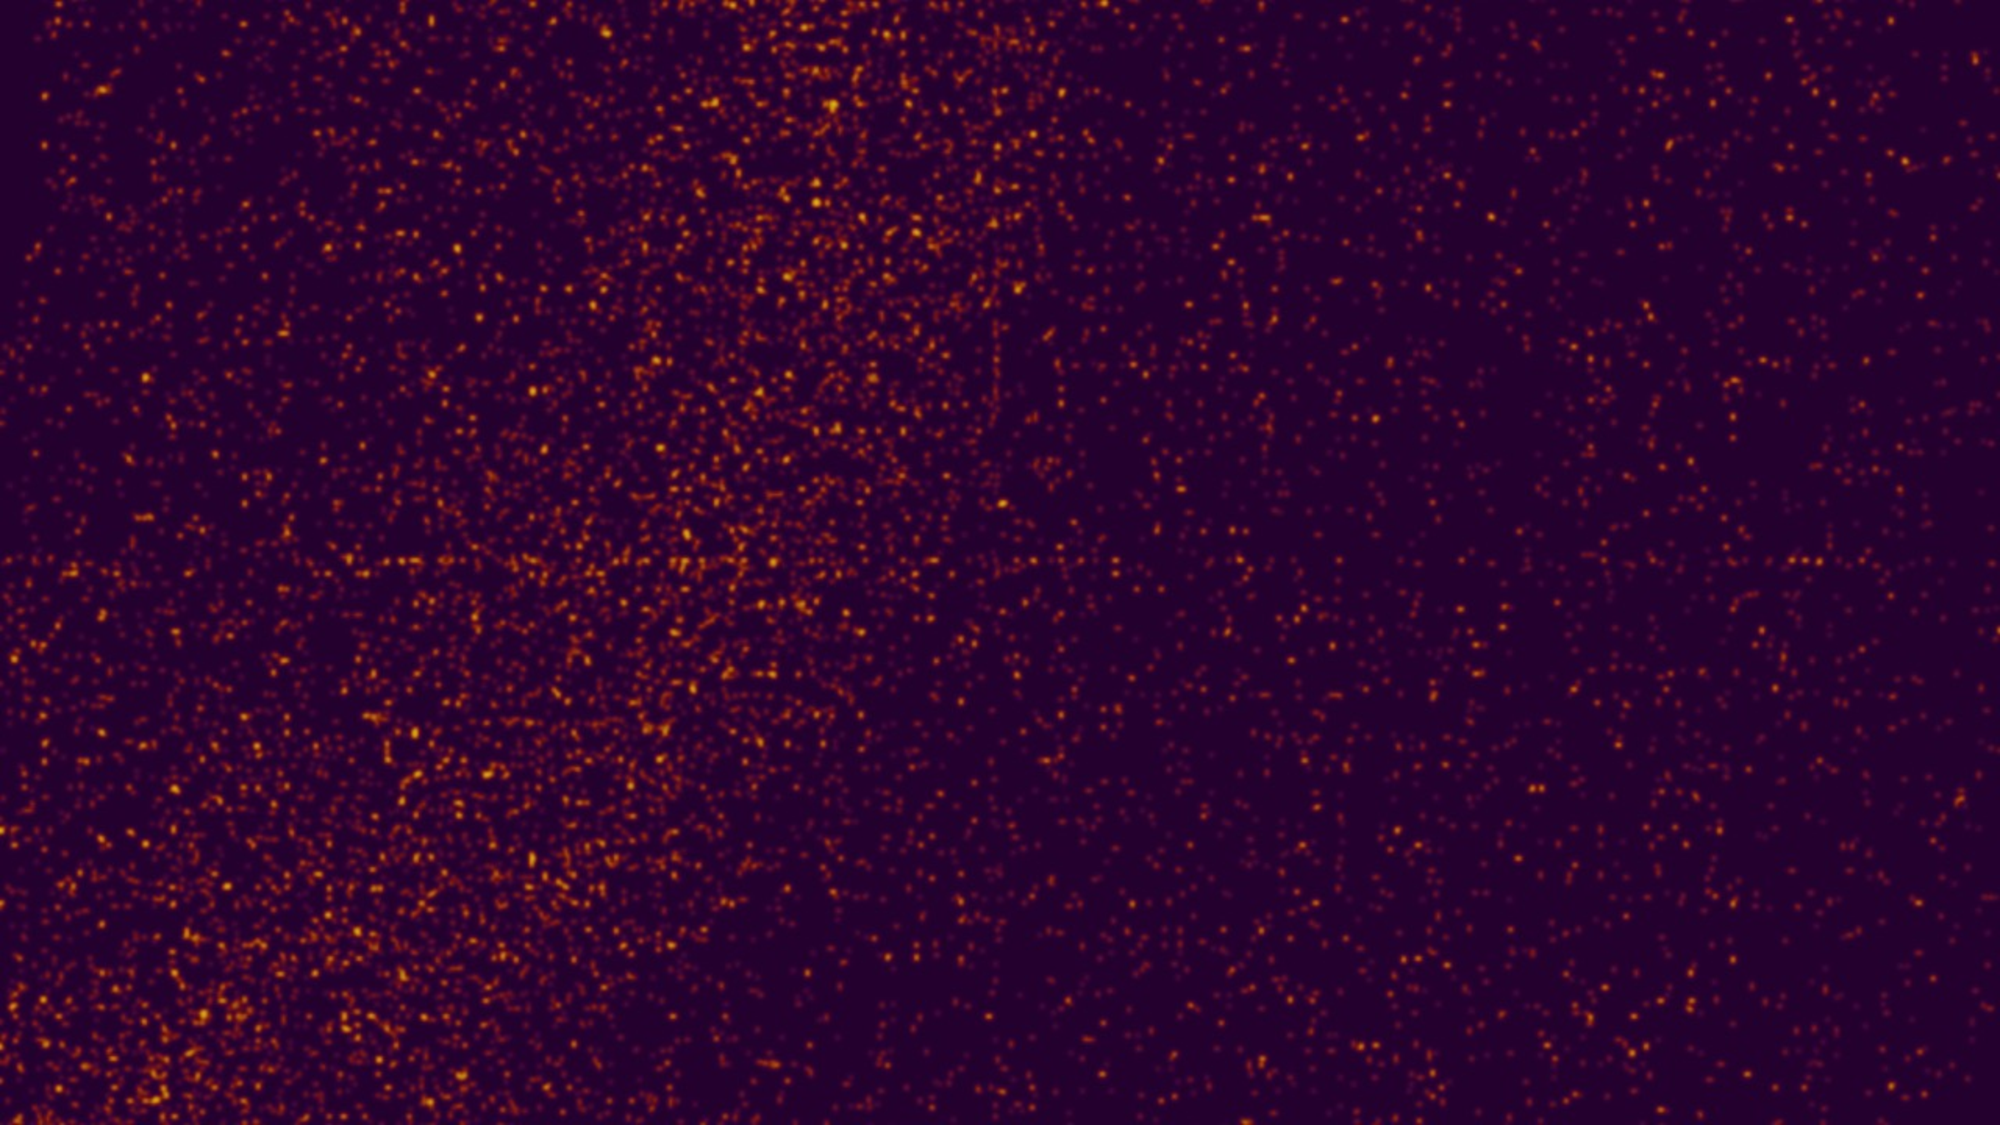
\includegraphics[width=1.2\linewidth]{./template/images/titlepage_background.pdf}}% Background/main image
    }
    \makeatletter
    \setbeamertemplate{title page}[default][left,colsep=-4bp] % align title page left
    \makeatother
    \setbeamerfont{title}{size=\@setfontsize\Huge{30}{20}}
    \setbeamercolor{title}{fg=white}
    \setbeamerfont{subtitle}{size=\@setfontsize\Huge{16}{12}}
    \setbeamercolor{subtitle}{fg=white}
    \setbeamercolor{author}{fg=white}
    \setbeamercolor{date}{fg=white}
    \setbeamercolor{institute}{fg=white}
    \setbeamertemplate{title page}{
        \vfill
        \begingroup
        \begin{groupcolumns}
            \hfill
            \begin{column}{0.65\textwidth}
                \usebeamertemplate{date}
                \usebeamertemplate*{title}
                \usebeamertemplate*{subtitle}
            \end{column}
            \begin{column}{0.35\textwidth}
                \usebeamertemplate*{titlegraphic}
            \end{column}
            \hfill
        \end{groupcolumns}
        \vspace{2pt}
        {\color{white}\hrule height 1pt}
        \usebeamertemplate{author}
        % \usebeamertemplate{institute}
        \vfill
        % Institutions at the bottom bar
        \vspace{10pt}
        \blackstrip{30pt}
        \vspace{-27pt}
        \includesvg[height=12pt]{./template/images/SLAC_TID_white.svg}
        {\color{white}\vrule width 0.1pt}
        \includesvg[height=12pt]{./template/images/TID_ID_IC.svg}
        \hfill
        \includesvg[height=12pt]{./template/images/Stanford_University.svg}
        {\color{white}\vrule width 0.1pt}
        \includesvg[height=12pt]{./template/images/DOE.svg}
        \vspace{4pt} % \vspace{-4pt}
        \endgroup
    }
}
\makeatother


% SloganTitleUnderline slide template
\makeatletter
\define@key{beamerframe}{SloganTitleUnderline}[true]{%
    \setbeamertemplate{frametitle}{%
        % \vskip-11.5pt % \vspace{-8.5pt}
        \vskip-11.5pt % \vspace{-8.5pt}
        \makebox[\textwidth]{
\includegraphics[width=\paperwidth]{./template/images/slogan.pdf}}
        \vskip-5pt%\vskip5.5pt 
        \usebeamerfont{frametitle}\huge\insertframetitle%
        \vphantom{g}% to avoid fluctuations per frame
        \vspace{3pt}% spacing between title text and horizontal line
        \hrule% 
        \vspace{-3pt}% adjust spacing after line
    }
    % \defaultfooter
}
\makeatother


% FloatingTitle (no underline) slide template
\makeatletter
\define@key{beamerframe}{FloatingTitle}[true]{%
    \setbeamertemplate{frametitle}{%
        \vskip-11.5pt % \vspace{-8.5pt}
        \makebox[\textwidth]{
\includegraphics[width=\paperwidth]{./template/images/slogan.pdf}}
        \vskip5.5pt
        \usebeamerfont{frametitle}\huge\insertframetitle%
        \vphantom{g}% to avoid fluctuations per frame
    }
    % \defaultfooter
}
\makeatother


% SectionTitlepage slide template
\makeatletter
\define@key{beamerframe}{SectionTitlepage}[true]{%
    \setbeamerfont{framesubtitle}{size=\@setfontsize\LARGE{12}{10}}
    \setbeamercolor{framesubtitle}{fg=stanford_black}%
    \setbeamertemplate{frametitle}{%
        \vskip-11.5pt % \vspace{-8.5pt}
        \makebox[\textwidth]{
\includegraphics[width=\paperwidth]{./template/images/slogan.pdf}}
        \vskip50pt
        {\color{stanford_black}\fontsize{35}{50}\selectfont\insertsectionnumber}
        \vskip6pt
        {\color{cardinal}\hrule height 0.5pt}
        \vskip15pt
        \usebeamerfont{frametitle}\Huge\insertframetitle%
        \vskip10pt
        \usebeamercolor[fg]{framesubtitle}\usebeamerfont{framesubtitle}\insertframesubtitle%
        \vphantom{g}% to avoid fluctuations per frame
    }
    % \defaultfooter
}
\makeatother


% TableOfContents (TOC) style
\setbeamertemplate{section in toc}[sections numbered]
% \setbeamerfont{section number projected}{size=\LARGE}
\setbeamerfont{section number projected}{size=\Large}
\setbeamercolor{section number projected}{bg=white,fg=black}

\setbeamertemplate{section in toc}{%
    \leavevmode\leftskip=4.75ex%1.75ex
  \llap{%
    \usebeamerfont*{section number projected}%
    \usebeamercolor[bg]{section number projected}%
    \vrule width2.25ex height1.85ex depth.4ex%
    \hskip-2.25ex%
    \hbox to2.25ex{\hfil\color{fg}\inserttocsectionnumber.\hfil}}%
\kern0.75ex\inserttocsection\par}

\makeatletter
\patchcmd{\beamer@sectionintoc}{\vskip1.5em}{\vskip0.5em}{}{}
% \patchcmd{\beamer@sectionintoc}{\vfill}{\vskip-0.2em}{}{} % reduce padding
% \patchcmd{\beamer@sectionintoc}{\vfill}{\vskip10pt}{}{} % reduce padding
\patchcmd{\beamer@sectionintoc}{\vfill}{\vskip1pt}{}{} % reduce padding
\makeatother






%%%%%%%%%%%%%%%%%%%%%%%%%%%%%%%%%%%%%%%%%%%%%%%%%%%%%%%%%%%%%%%%%%%%%%%%%%%%%%%%
%%%%%%%%%%%%%%%%%%%%%%%%%%%%%%%%%%%%%%%%%%%%%%%%%%%%%%%%%%%%%%%%%%%%%%%%%%%%%%%%
%%%%%%%%%%%%%%%%%%%%%%%%%%%%%%%%%%%%%%%%%%%%%%%%%%%%%%%%%%%%%%%%%%%%%%%%%%%%%%%%

\begin{document}


\begin{frame}[Titlepage, plain, noframenumbering]
\titlepage
\end{frame}

\begin{frame}{Introduction}
  \begin{columns}
      \begin{column}{0.5\textwidth}
        \begin{itemize}
            \item Llorenç Fanals-i-Batllori.
            \item BSc EE Universitat the Girona, Spain (9.52/10), MSc EE UPC Barcelona, Spain (9.69/10).
            \item Mixed-signal Design Verification Engineer at Apple, UK.
            \item Mixed-signal ASIC Design Engineer at SLAC/Stanford.
        \end{itemize}
      \end{column}
      \begin{column}{0.5\textwidth}
        \begin{figure} \centering
            
\includegraphics[width=0.8\textwidth]{./images/portrait_.jpeg}
        \end{figure}
      \end{column}
  \end{columns}
\end{frame}

\begin{frame}[SloganTitleUnderline]{Table of contents}
    \LARGE \tableofcontents%[section]
\end{frame}



%%%%%%%%%%%%%%%%%%%%%%%%%%%%%%%%%%%%%%%%%%%%%%%%%%%%%%%%%%%%%%%%%%%%%%%%%%%%%%%%
% 1: Cryogenic systems
%%%%%%%%%%%%%%%%%%%%%%%%%%%%%%%%%%%%%%%%%%%%%%%%%%%%%%%%%%%%%%%%%%%%%%%%%%%%%%%%
\section{Cryogenic systems}
\begin{frame}[SectionTitlepage]{Cryo-CMOS power management}
\end{frame}

\begin{frame}{Cryo-CMOS power management}
\end{frame}

\subsection{Cryo-CMOS power management sub}
\begin{frame}[SectionTitlepage]{Cryo-CMOS power management}
\end{frame}





% %%%%%%%%%%%%%%%%%%%%%%%%%%%%%%%%%%%%%%%%%%%%%%%%%%%%%%%%%%%%%%%%%%%%%%%%%%%%%%%%
% % 1: Silicon bring-up
% %%%%%%%%%%%%%%%%%%%%%%%%%%%%%%%%%%%%%%%%%%%%%%%%%%%%%%%%%%%%%%%%%%%%%%%%%%%%%%%%
% % \section{Silicon bring-up}
% % \begin{frame}[SectionTitlepage]{Silicon bring-up}
% % \end{frame}
% 
% \begin{frame}{Silicon bring-up}
%     You just received your ASICs. Now what?
% %     \begin{enumerate}
% %         \item PCB design.
% %         \item Packaging (wire bonding).
% %         \item Sanity checks.
% %         \item Power-up.
% %         \item Characterization.
% %     \end{enumerate}
% \end{frame}
% 
% \begin{frame}{Hand it off?}
%     \begin{figure} \centering
%         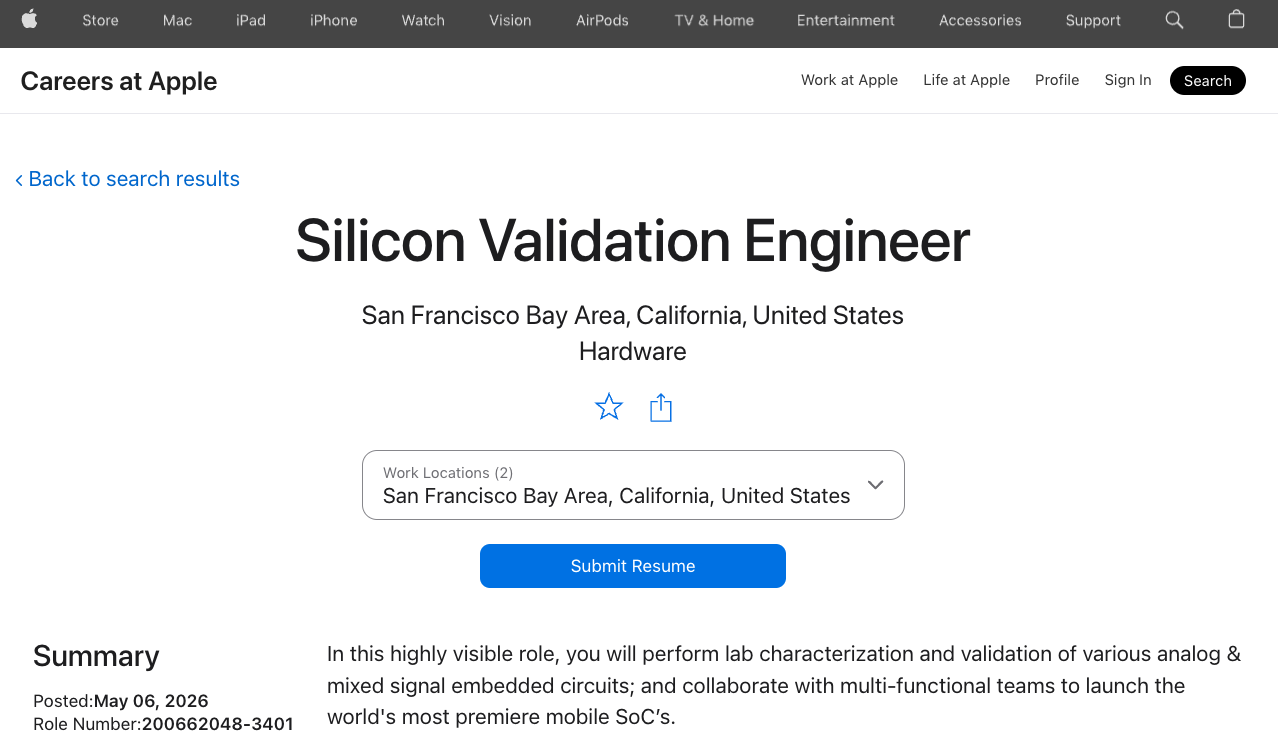
\includegraphics[width=0.8\textwidth]{./images/SiVal2.png}
%     \end{figure}
% \end{frame}
% 
% \begin{frame}{Silicon bring-up}
%     You just received your ASICs. Now what?
%     \begin{enumerate}
%         \item PCB design.
%         \item Packaging (wire bonding).
%         \item Embedded system.
%         \item Sanity checks.
%         \item Power-up.
%         \item Characterization.
%     \end{enumerate}
% \end{frame}
% 
% \begin{frame}{Do it yourself!}
%     \begin{figure} \centering
%         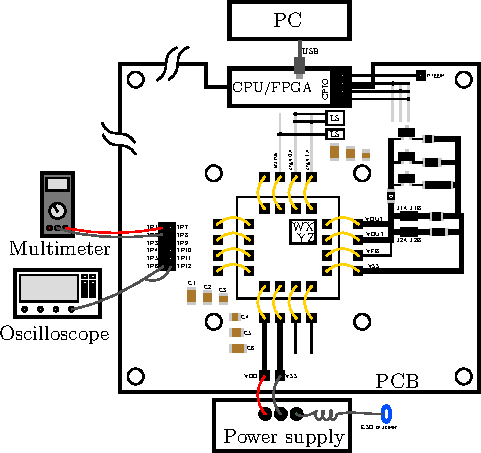
\includegraphics[width=0.55\textwidth]{./figures/big.pdf}
%     \end{figure}
% \end{frame}
% 
% \begin{frame}{General advice}
%     \begin{itemize}
%         \item Document.
%         \item Use version control (git).
%         \item Use redundancy, avoid a single point of failure.
%         \item Print in paper your pinout (ASIC and PCB).
%         \item Wear an ESD bracelet.
%     \end{itemize}
% \end{frame}
% 
% 
% 
% %%%%%%%%%%%%%%%%%%%%%%%%%%%%%%%%%%%%%%%%%%%%%%%%%%%%%%%%%%%%%%%%%%%%%%%%%%%%%%%%
% \section{PCB design}
% \begin{frame}[SectionTitlepage]{PCB design}
% \end{frame}
% %%%%%%%%%%%%%%%%%%%%%%%%%%%%%%%%%%%%%%%%%%%%%%%%%%%%%%%%%%%%%%%%%%%%%%%%%%%%%%%%
% \begin{frame}{PCB design}
%     \begin{figure} \centering
%         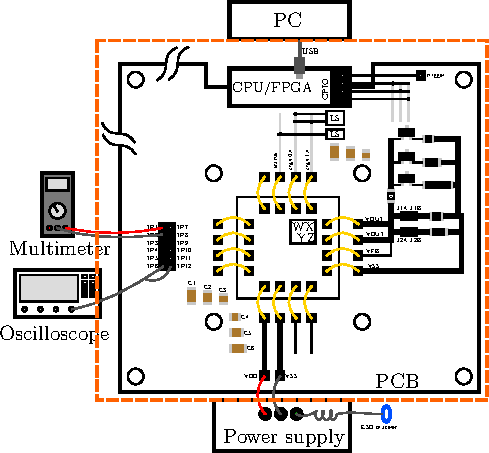
\includegraphics[width=0.55\textwidth]{./figures/bigh_pcb.pdf}
%     \end{figure}
% \end{frame}
% 
% \begin{frame}{PCB design}
%     Potentials software to use:
%     \begin{itemize}
%         \item Altium: profressional-grade, needs a license.
%         \item KiCad: "hobbyist" software but extremely capable as of 2026.
%         \item EasyEDA: limited capabilities but smooth integration with PCB manufacturer.
%     \end{itemize}
%   \begin{columns}
%       \begin{column}{0.3\textwidth}
%         \begin{figure} \centering
%             
\includegraphics[width=0.9\textwidth]{./images/altium.jpg}
%         \end{figure}
%       \end{column}
%       \begin{column}{0.3\textwidth}
%         \begin{figure} \centering
%             
\includegraphics[width=0.9\textwidth]{./images/kicad.jpg}
%         \end{figure}
%       \end{column}
%       \begin{column}{0.3\textwidth}
%         \begin{figure} \centering
%             
\includegraphics[width=0.9\textwidth]{./images/easyeda.png}
%         \end{figure}
%       \end{column}
%   \end{columns}
% 
% \end{frame}
% 
% 
% \begin{frame}{PCB design I}
%   \vspace{-0.3cm}
%   \begin{columns}
%       \hspace{0.4cm}
%       \begin{column}{0.45\textwidth}
%         Obtain the sheet resistance of the conducting metal, in \SI{}{\ohm\per\square}.
%         \begin{enumerate}
%             \item Design to minimize voltage drop $IR$ on nets that carry current.
%             \item Nets driving a high-impedance pin (transistor gate) are much more relaxed. Make them minimum dimensions ($\sim$ 4 mil).
%         \end{enumerate}
%       \end{column}
%       \begin{column}{0.52\textwidth}
%         \begin{figure} \centering
%             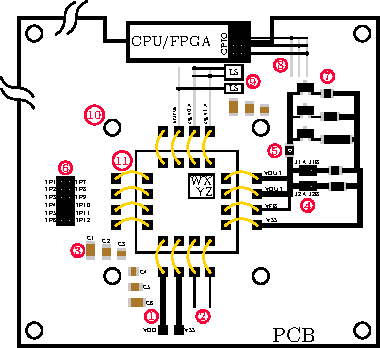
\includegraphics[width=0.9\textwidth]{./figures/big_pcb.pdf}
%         \end{figure}
%       \end{column}
%   \end{columns}
% \end{frame}
% 
% \begin{frame}{PCB design II}
%   \vspace{-0.3cm}
%   \begin{columns}
%       \hspace{0.4cm}
%       \begin{column}{0.45\textwidth}
%         \begin{enumerate}
%             \setcounter{enumi}{2}
%             \item Use decoupling capacitors between supply and ground. Use different cap values to improve the frequency response (or not \cite{rosenberg_decoupling}).
%             \item Use jumpers to increase flexibility during testing.
%             \item Or 0-Ohm resistors.
%             \item Place extensive test points. There must be a good reason for a PCB net to not be exposed/measurable. Label them.
%         \end{enumerate}
%       \end{column}
%       \begin{column}{0.52\textwidth}
%         \begin{figure} \centering
%             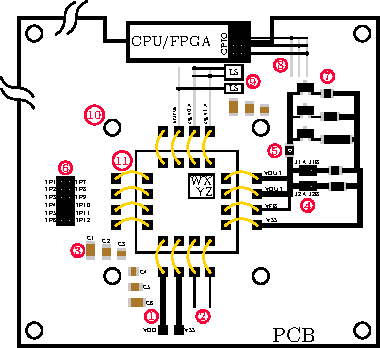
\includegraphics[width=0.9\textwidth]{./figures/big_pcb.pdf}
%         \end{figure}
%       \end{column}
%   \end{columns}
% \end{frame}
% 
% \begin{frame}{PCB design III}
%   \vspace{-0.3cm}
%   \begin{columns}
%       \hspace{0.4cm}
%       \begin{column}{0.45\textwidth}
%         \begin{enumerate}
%             \setcounter{enumi}{6}
%             \item You can place an array of binary-weighted resistors and small $R_{DS}$ MOSFETs to realize a tunable load. The gate voltages may need a level shifter (LS). Be aware of the GPIO latency.
%             \item Use metals at different levels in an orthogonal fashion.
%             \item Level shifters (LS) are needed to accommodate the ASIC voltage domain to that of the GPIOs, and viceversa.
%         \end{enumerate}
%       \end{column}
%       \begin{column}{0.52\textwidth}
%         \begin{figure} \centering
%             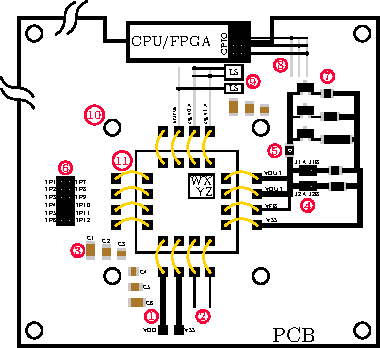
\includegraphics[width=0.9\textwidth]{./figures/big_pcb.pdf}
%         \end{figure}
%       \end{column}
%   \end{columns}
% \end{frame}
% 
% \begin{frame}{PCB design IV}
%   \vspace{-0.3cm}
%   \begin{columns}
%       \hspace{0.4cm}
%       \begin{column}{0.45\textwidth}
%         \begin{enumerate}
%             \setcounter{enumi}{9}
%             \item Place mounting holes both at the PCB level and around the ASIC.
%             \item Give a separation between PCB pads and ASIC of \SI{300}{\um} at least. A special surface finish may be needed.
%         \end{enumerate}
%       \end{column}
%       \begin{column}{0.52\textwidth}
%         \begin{figure} \centering
%             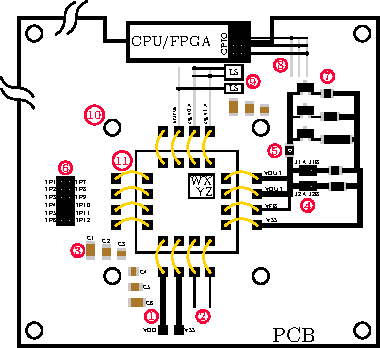
\includegraphics[width=0.9\textwidth]{./figures/big_pcb.pdf}
%         \end{figure}
%       \end{column}
%   \end{columns}
% \end{frame}
% 
% \begin{frame}{PCB design: example I (Andrew Young)}
%     \vspace{-0.6cm}
%   \begin{columns}
%       \hspace{0.4cm}
%       \begin{column}{0.45\textwidth}
%         \begin{figure} \centering
%             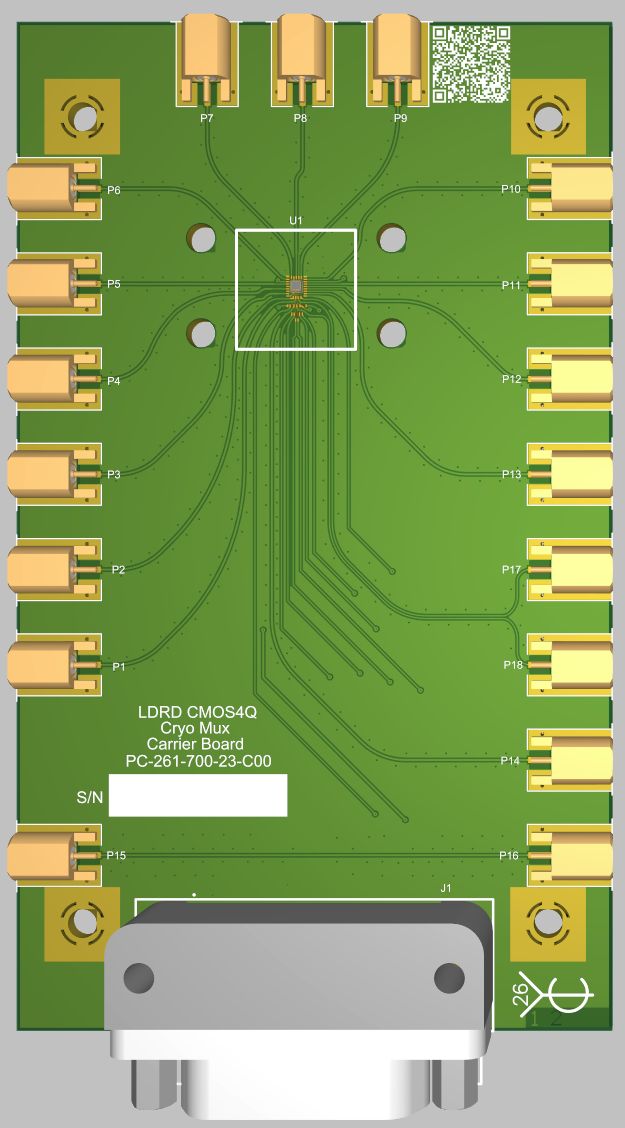
\includegraphics[height=0.8\textheight]{./images/C4Q1_carrier_render.png}
%         \end{figure}
%       \end{column}
%       \begin{column}{0.45\textwidth}
%         \begin{figure} \centering
%             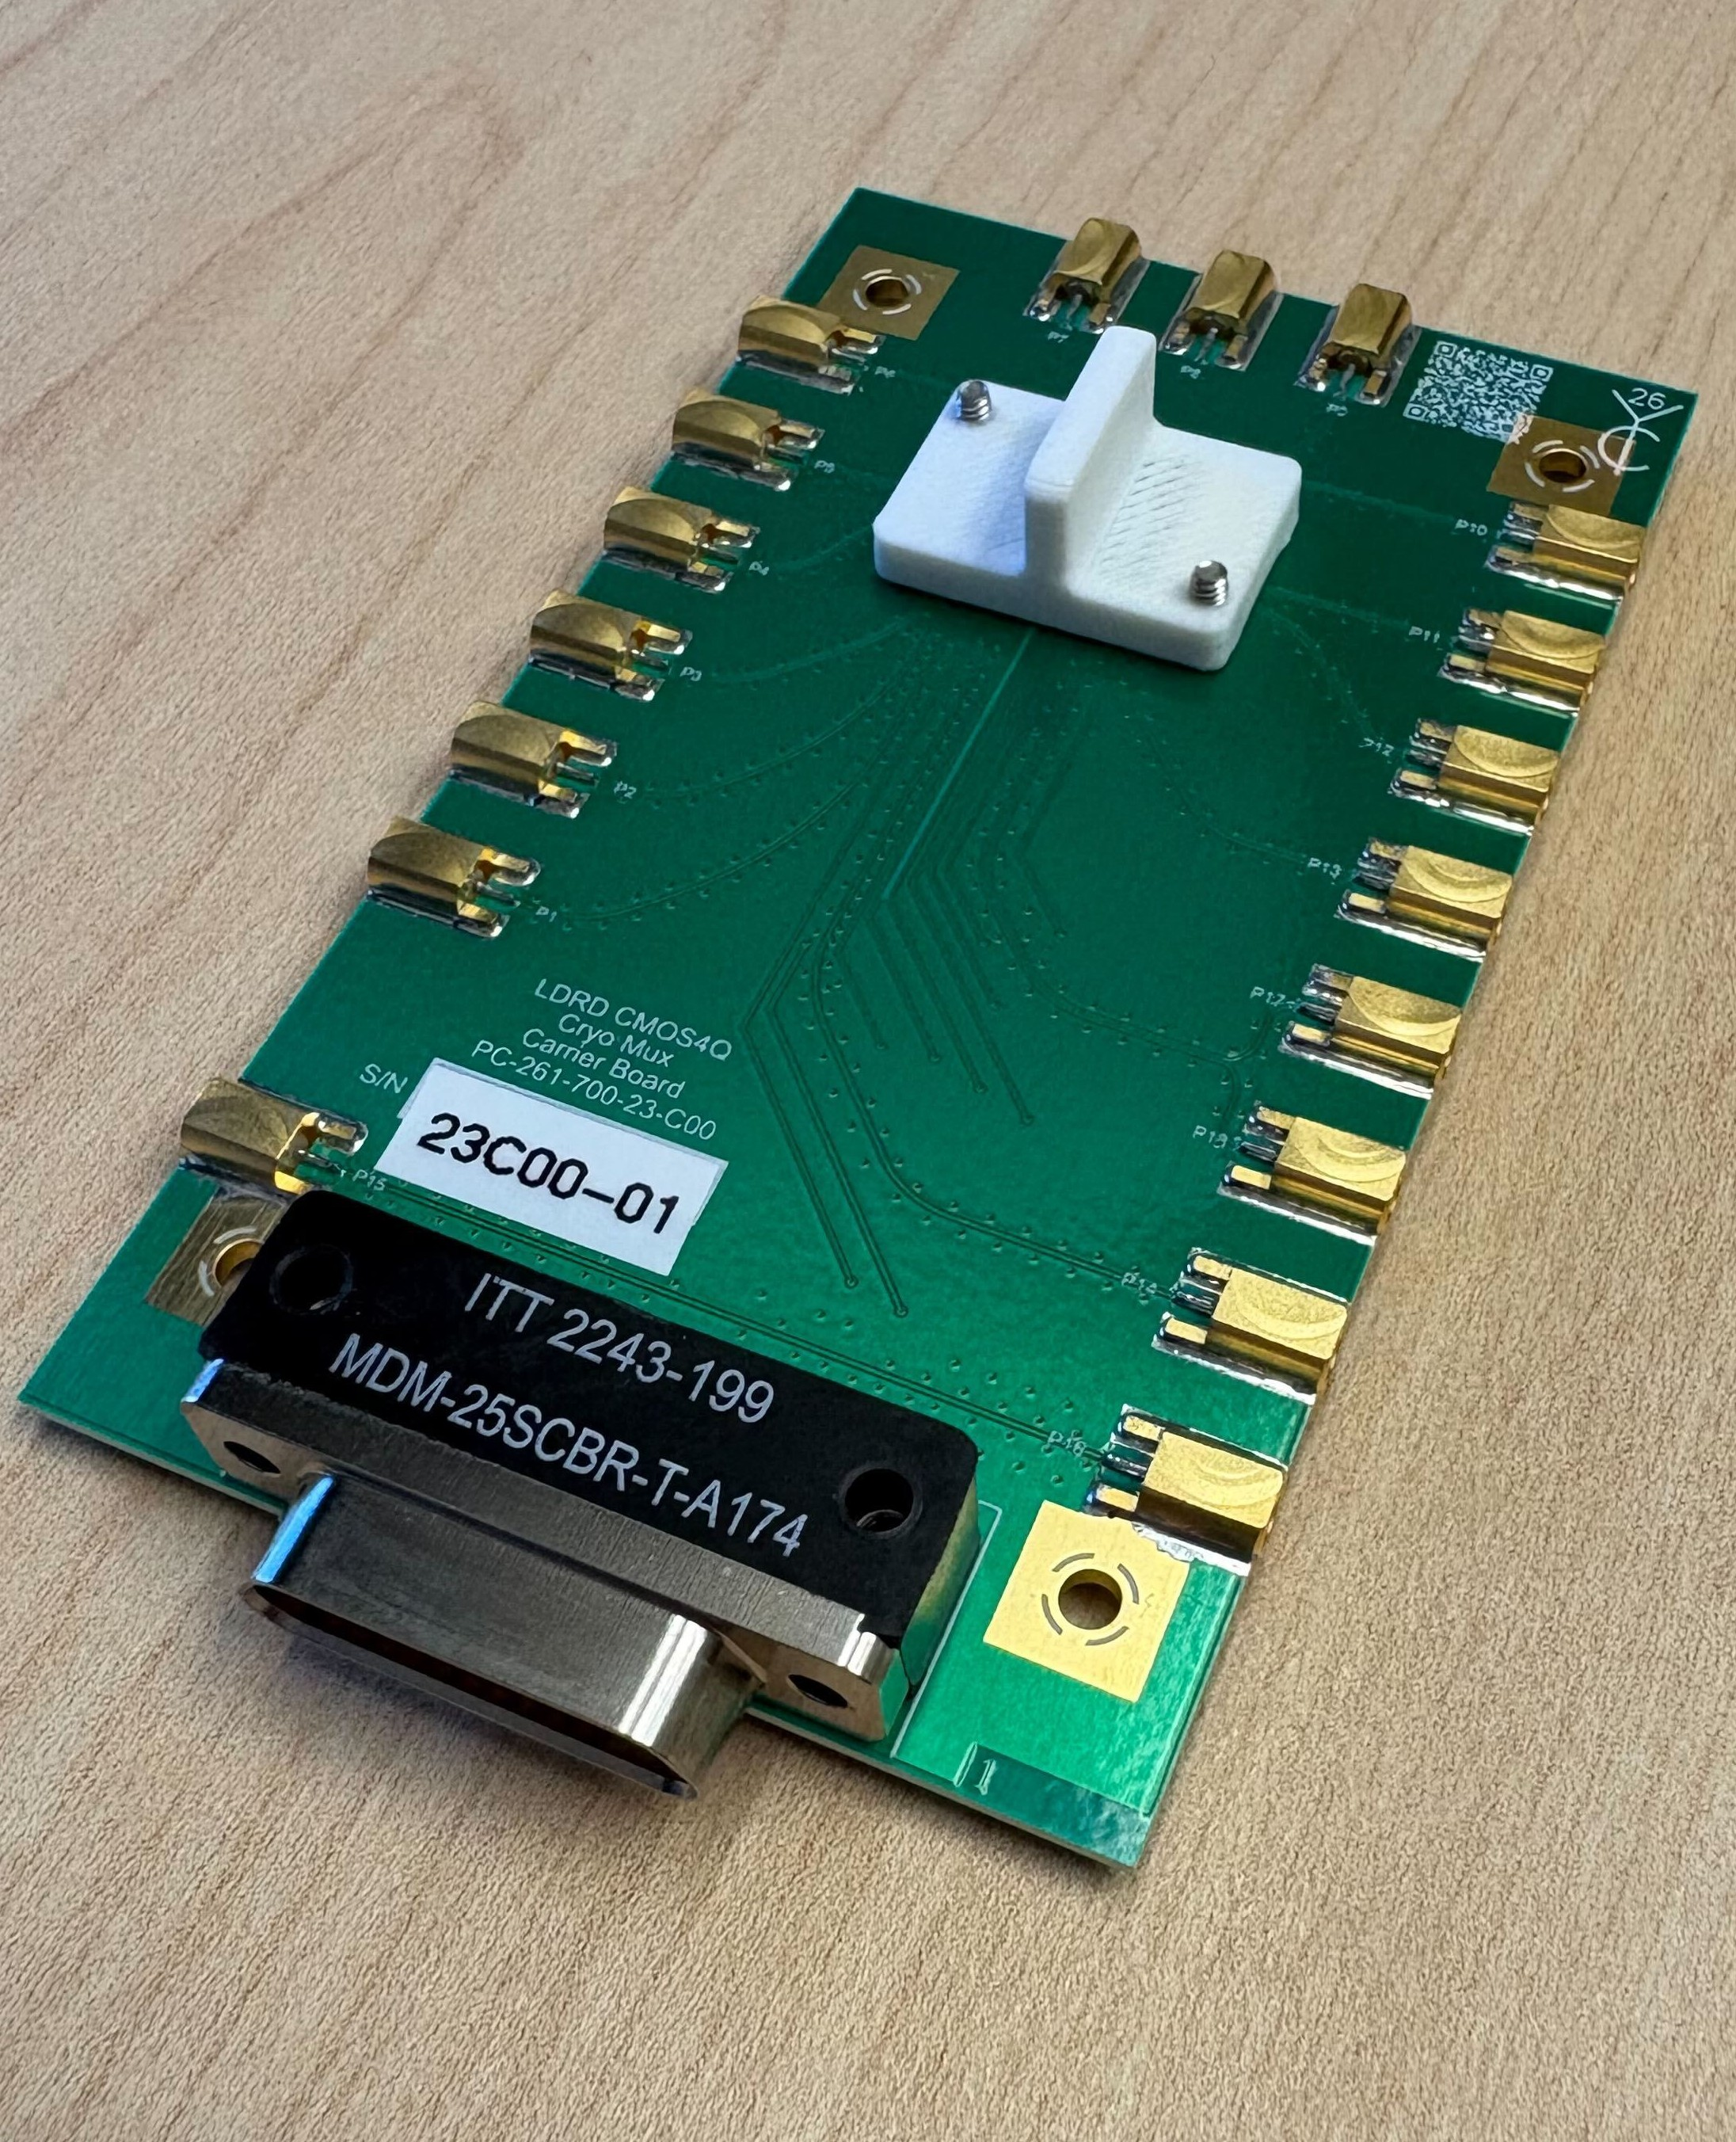
\includegraphics[height=0.8\textheight]{./images/C4Q1_carrier_pic.jpg}
%         \end{figure}
%       \end{column}
%   \end{columns}
% \end{frame}
% 
% \begin{frame}{PCB design: example II (Joan Serrano Aporta)}
%     \begin{figure} \centering
%         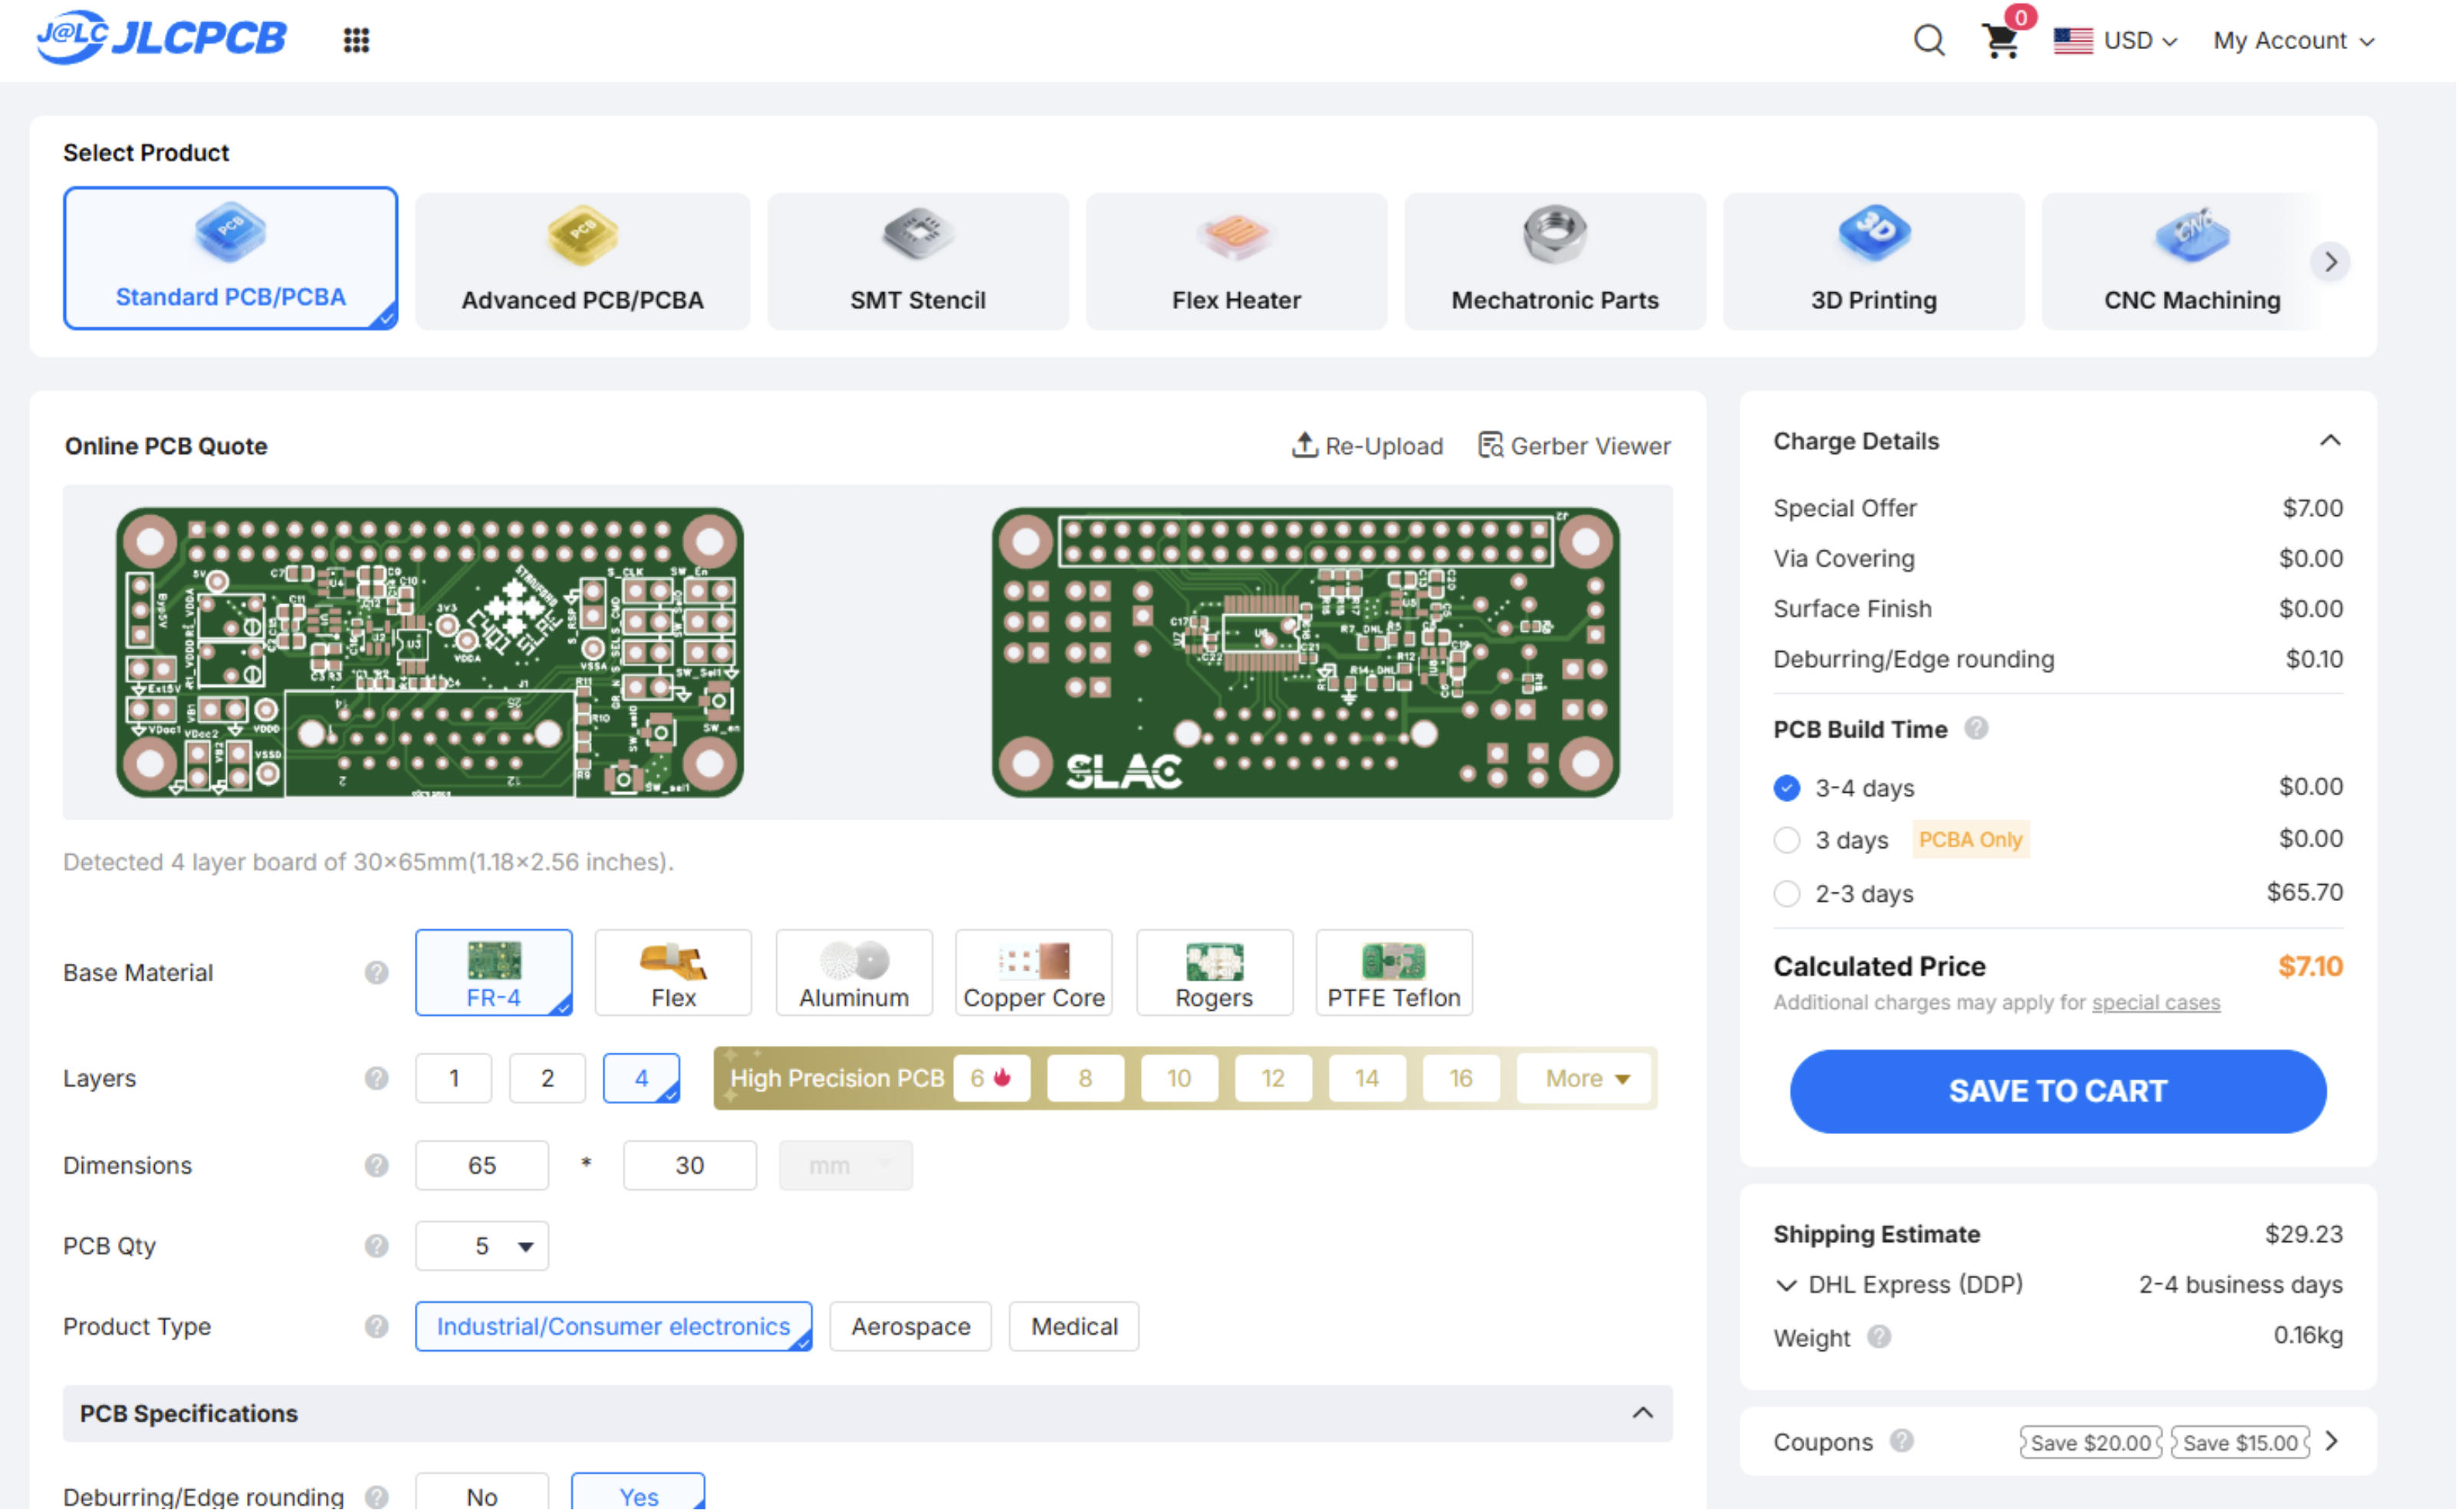
\includegraphics[width=0.8\textwidth]{./images/pcb_C4Q1_interface_jlcpcb.png}
%     \end{figure}
% \end{frame}
% 
% \begin{frame}{PCB design: example II (Joan Serrano Aporta)}
%     \vspace{-0.5cm}
%   \begin{columns}
%       \hspace{0.4cm}
%       \begin{column}{0.45\textwidth}
%           \begin{itemize}
%             \item Total cost: $\sim 350 \$$, 5 boards, entirely populated.
%             \item Turnaround time: 1 week.
%             \item No issues observed.
%           \end{itemize}
%       \end{column}
%       \begin{column}{0.45\textwidth}
%         \begin{figure} \centering
%             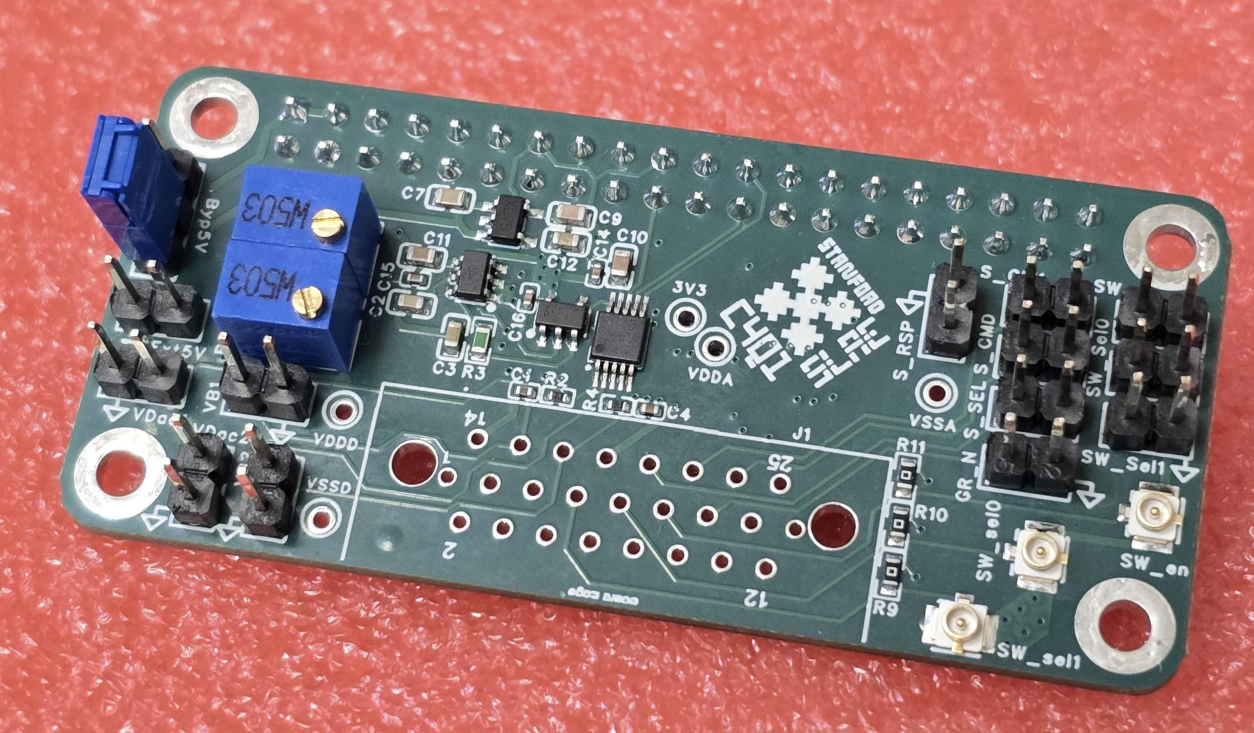
\includegraphics[width=0.9\textwidth]{./images/pcb_C4Q1_interface_pic_one.png}
%         \end{figure}
%         \begin{figure} \centering
%             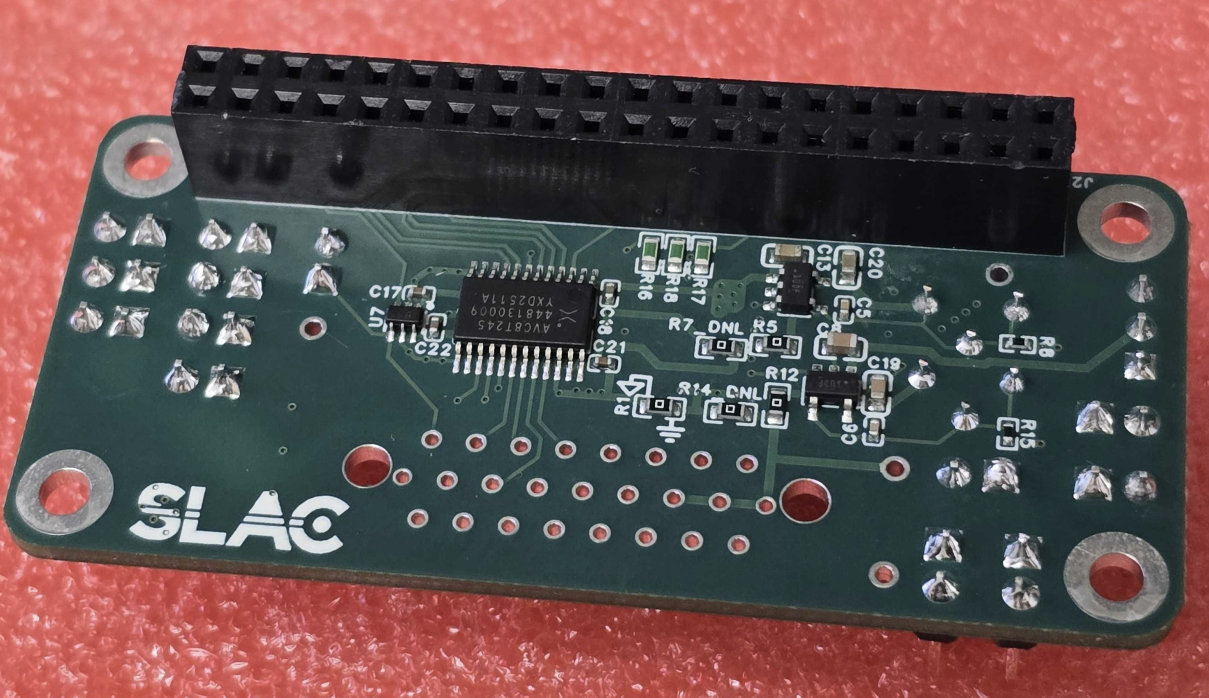
\includegraphics[width=0.9\textwidth]{./images/pcb_C4Q1_interface_pic_two.png}
%         \end{figure}
%       \end{column}
%   \end{columns}
% \end{frame}
% 
% 
% 
% 
% %%%%%%%%%%%%%%%%%%%%%%%%%%%%%%%%%%%%%%%%%%%%%%%%%%%%%%%%%%%%%%%%%%%%%%%%%%%%%%%%
% \section{Packaging (wire bonding)}
% \begin{frame}[SectionTitlepage]{Packaging (wire bonding)}
% \end{frame}
% %%%%%%%%%%%%%%%%%%%%%%%%%%%%%%%%%%%%%%%%%%%%%%%%%%%%%%%%%%%%%%%%%%%%%%%%%%%%%%%%
% \begin{frame}{Packaging (wire bonding)}
%     \begin{figure} \centering
%         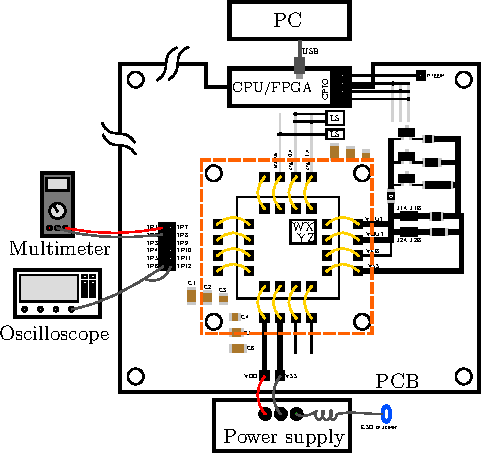
\includegraphics[width=0.55\textwidth]{./figures/bigh_bond.pdf}
%     \end{figure}
% \end{frame}
% 
% \begin{frame}{ESD bracelet}
%   \begin{columns}
%       \begin{column}{0.45\textwidth}
%         \begin{figure} \centering
%             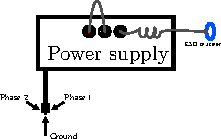
\includegraphics[width=0.9\textwidth]{./figures/esd_bracelet.pdf}
%         \end{figure}
%       \end{column}
%       \begin{column}{0.52\textwidth}
%         \begin{figure} \centering
%             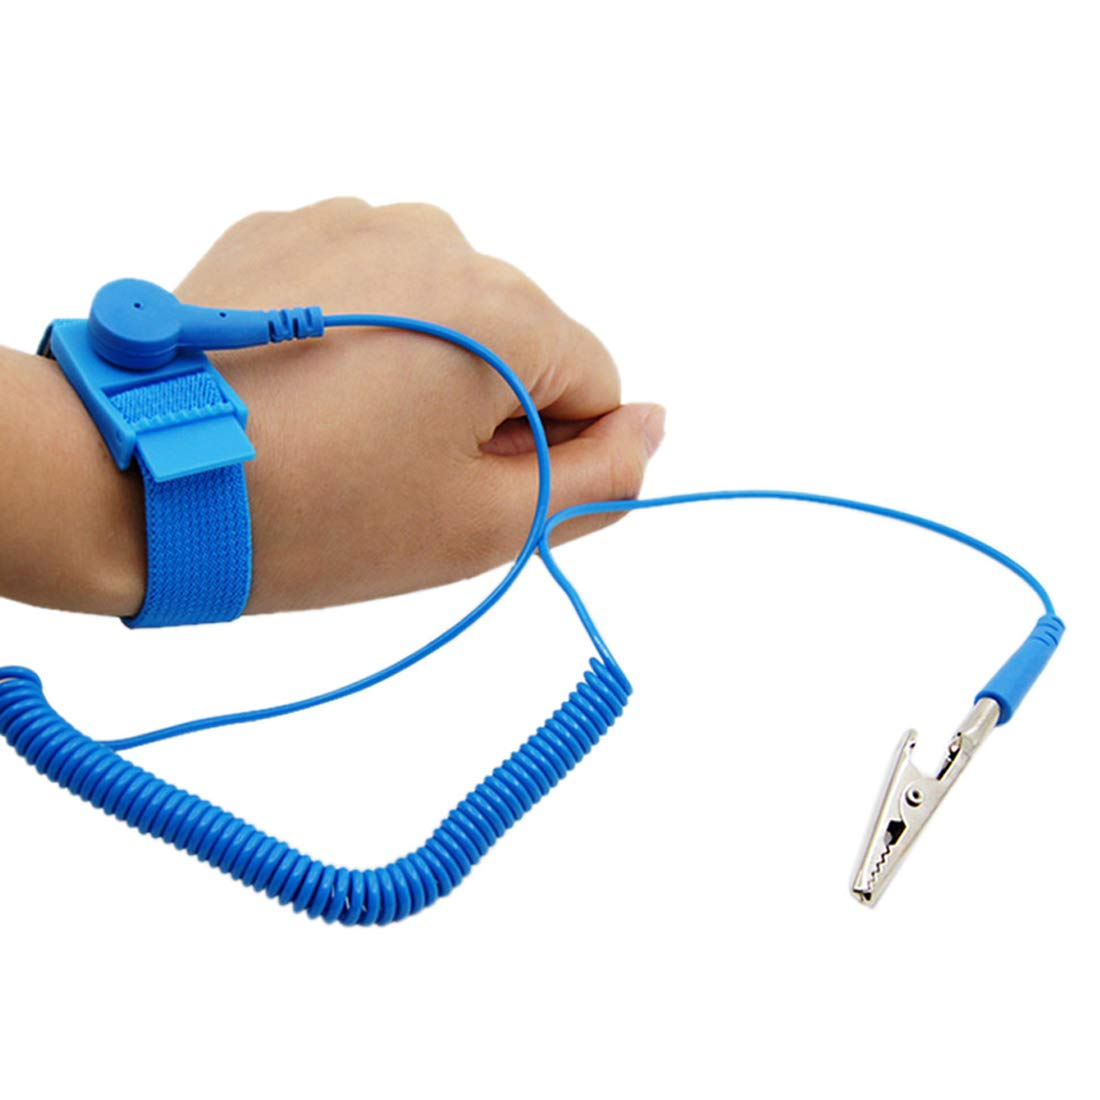
\includegraphics[width=0.9\textwidth]{./images/esd_bracelet.jpg}
%         \end{figure}
%       \end{column}
%   \end{columns}
% \end{frame}
% 
% \begin{frame}{ESD bracelet}
%   \begin{columns}
%       \begin{column}{0.45\textwidth}
%         \begin{figure} \centering
%             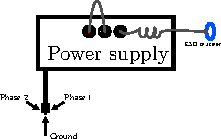
\includegraphics[width=0.9\textwidth]{./figures/esd_bracelet.pdf}
%         \end{figure}
%       \end{column}
%       \begin{column}{0.52\textwidth}
%         \begin{figure} \centering
%             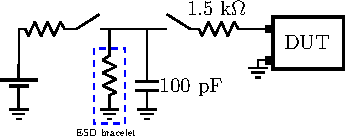
\includegraphics[width=0.9\textwidth]{./figures/hbm.pdf}
%         \end{figure}
%       \end{column}
%   \end{columns}
% \end{frame}
% 
% 
% \begin{frame}{Packaging (wire bonding)}
%   \vspace{-0.3cm}
%   \begin{columns}
%       \hspace{0.4cm}
%       \begin{column}{0.45\textwidth}
%         \begin{enumerate}
%             \item Give clear indications of the ASIC orientation. A logo or a disctinctive feature can be extremely helpful.
%             \item Be aware of the $\sim \SI{1}{\nH\per\mm}$ series inductance. Keep supply and analog bonds as short as possible.
%             \item Provide sufficient spacing between PCB pads and ASIC pads.
%             \item Make the PCB pad large enough while meeting DRC rules.
%         \end{enumerate}
%       \end{column}
%       \begin{column}{0.52\textwidth}
%         \begin{figure} \centering
%             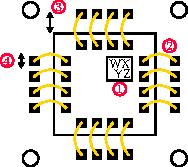
\includegraphics[width=0.9\textwidth]{./figures/big_wirebonding.pdf}
%         \end{figure}
%       \end{column}
%   \end{columns}
% \end{frame}
% 
% \begin{frame}{Wire bonding: example I (Matt Cherry)}
%     \begin{figure} \centering
%         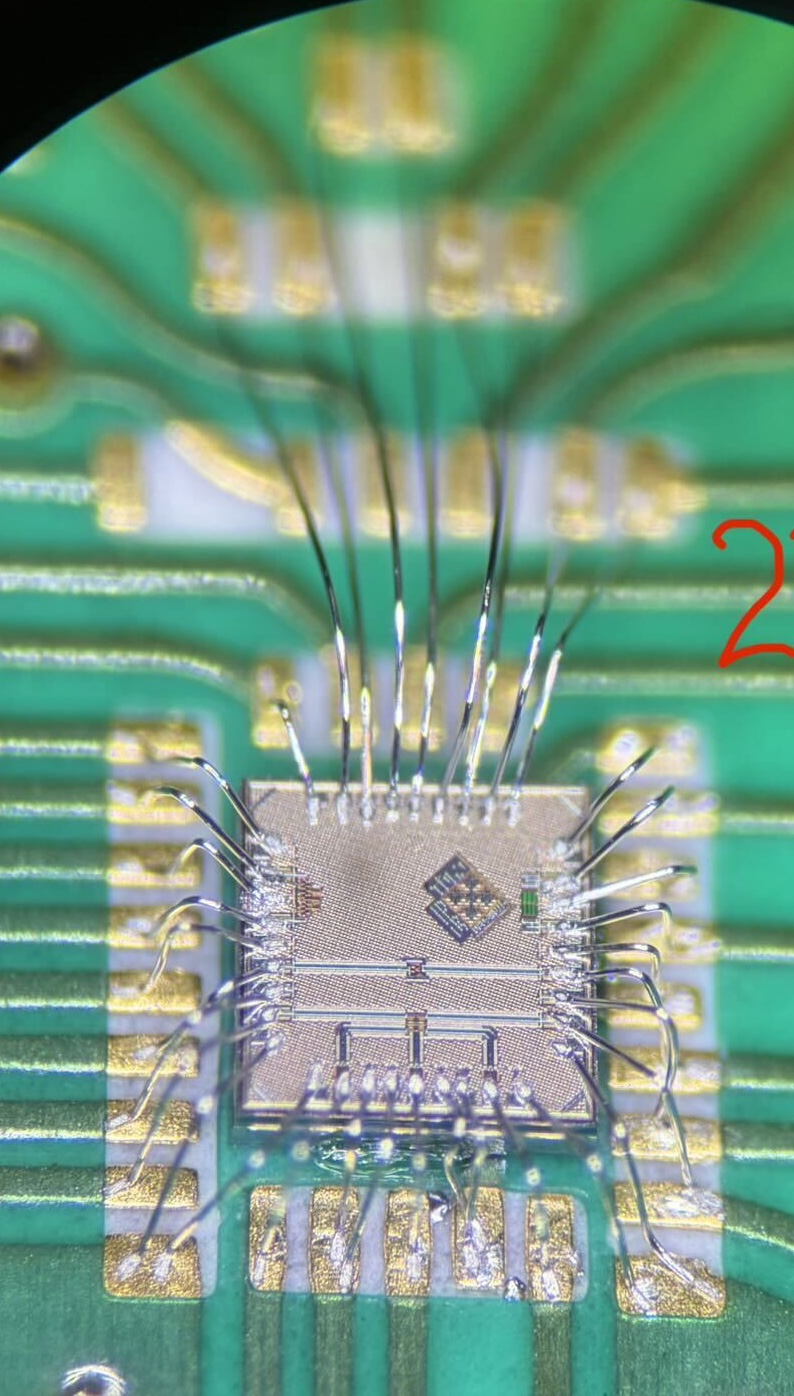
\includegraphics[width=0.3\textwidth]{./images/C4Q1_22_.jpg}
%     \end{figure}
% \end{frame}
% 
% \begin{frame}{Wire bonding: example II (Matt Cherry)}
%     \begin{figure} \centering
%         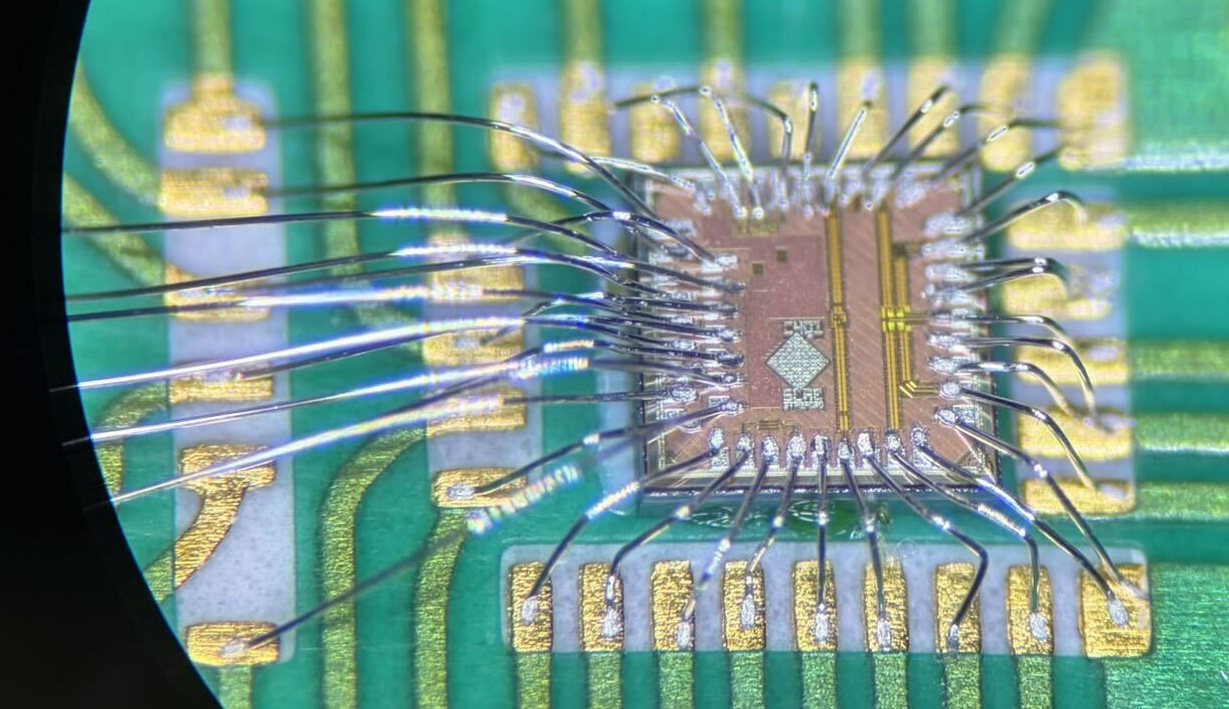
\includegraphics[width=0.8\textwidth]{./images/C4Q1_28_.jpg}
%     \end{figure}
% \end{frame}
% 
% 
% %%%%%%%%%%%%%%%%%%%%%%%%%%%%%%%%%%%%%%%%%%%%%%%%%%%%%%%%%%%%%%%%%%%%%%%%%%%%%%%%
% \section{Embedded system}
% \begin{frame}[SectionTitlepage]{Embedded system}
% \end{frame}
% %%%%%%%%%%%%%%%%%%%%%%%%%%%%%%%%%%%%%%%%%%%%%%%%%%%%%%%%%%%%%%%%%%%%%%%%%%%%%%%%
% 
% \begin{frame}{Embedded system}
%     \begin{figure} \centering
%         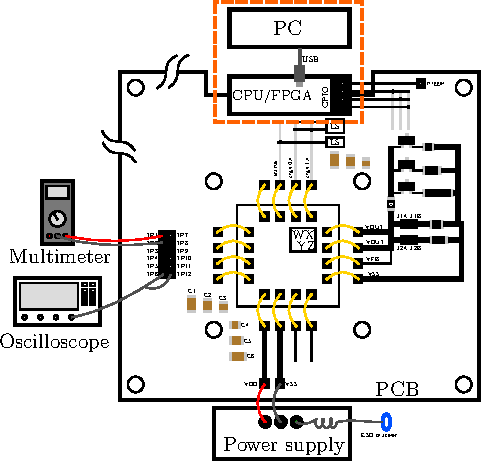
\includegraphics[width=0.55\textwidth]{./figures/bigh_embedded.pdf}
%     \end{figure}
% \end{frame}
% 
% \begin{frame}{Raspberry Pi}
%     \begin{figure} \centering
%         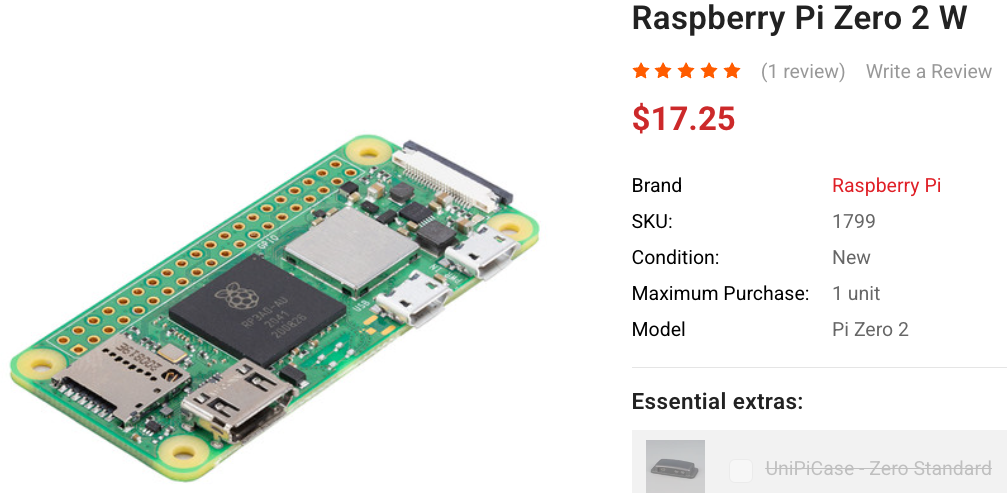
\includegraphics[width=0.5\textwidth]{./images/RPi_buy.png}
%     \end{figure}
%     \begin{itemize}
%         \item A Linux system with GPIOs for $20 \$$.
%         \item Can run Claude on it!
%         \item Do not use for deterministic / precise timing operations.
%         \item Be careful about noise.
%     \end{itemize}
% \end{frame}
% 
% \begin{frame}{Raspberry Pi interface}
%     \texttt{picocom -b 115200 /dev/cu.usbmodem11103}
%     \begin{figure} \centering
%         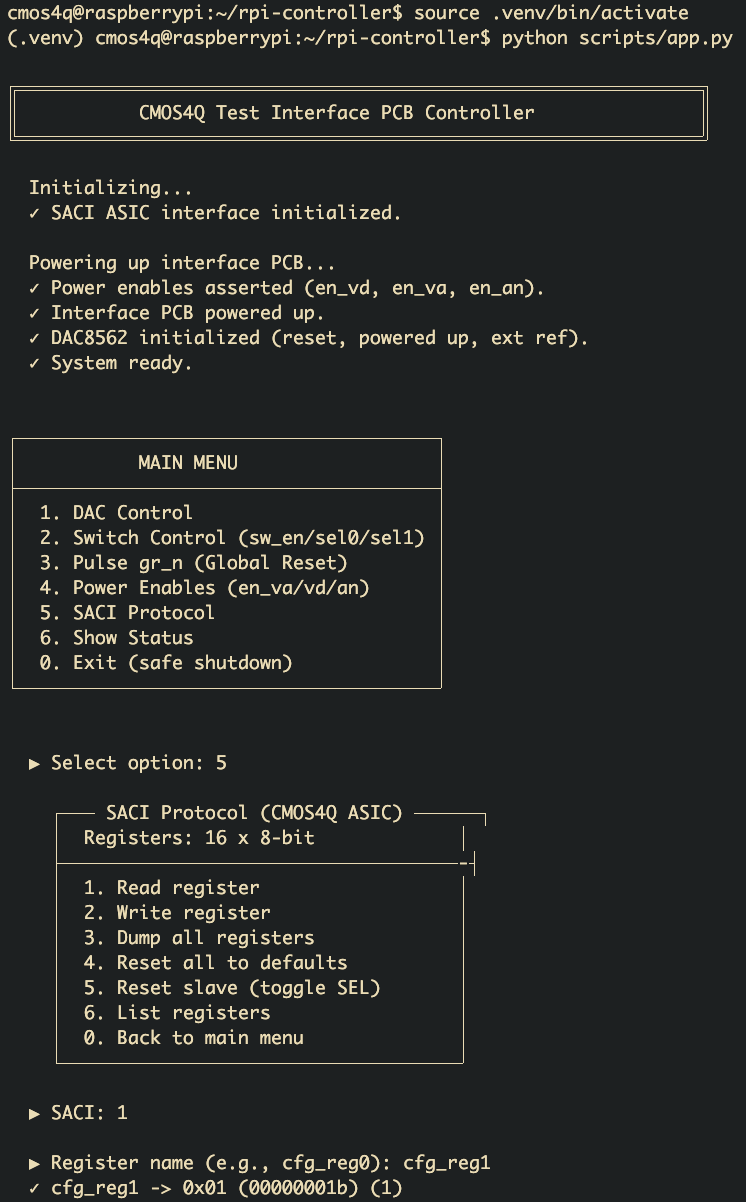
\includegraphics[width=0.28\textwidth]{./images/RPi_menu.png}
%     \end{figure}
% \end{frame}
% 
% \begin{frame}{Arduino}
%     \begin{figure} \centering
%         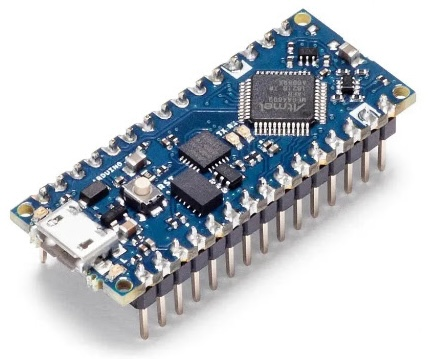
\includegraphics[width=0.3\textwidth]{./images/arduino_nano.jpg}
%     \end{figure}
%     \begin{itemize}
%         \item A microcontroller.
%         \item C code gets mapped into assembly, so real-time operation.
%         \item Not interactive by default.
%     \end{itemize}
% \end{frame}
% 
% \begin{frame}{LabVIEW-based DAQ}
% \vspace{-0.8cm}
%   \begin{columns}
%       \begin{column}{0.3\textwidth}
%         \begin{figure} \centering
%             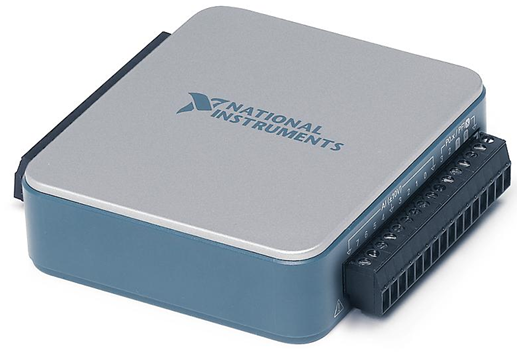
\includegraphics[width=0.9\textwidth]{./images/NI_IO.png}
%         \end{figure}
%       \end{column}
%       \begin{column}{0.7\textwidth}
%         \begin{figure} \centering
%             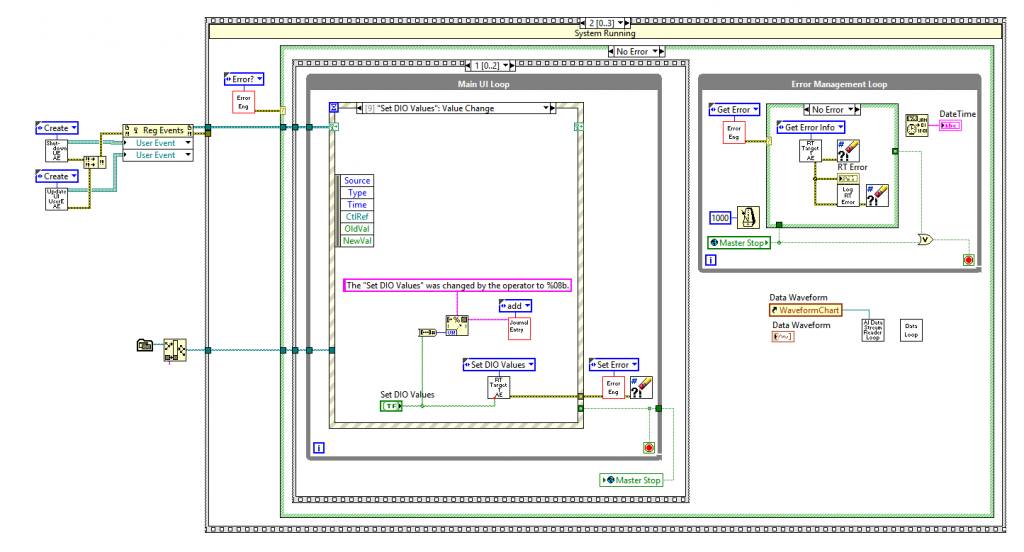
\includegraphics[width=0.99\textwidth]{./images/LabView.png}
%         \end{figure}
%       \end{column}
%   \end{columns}
%     \begin{itemize}
%         \item Expensive.
%         \item Could digitize the LDO output.
%         \item Can synchronize events.
%     \end{itemize}
% \end{frame}
% 
% 
% 
% %%%%%%%%%%%%%%%%%%%%%%%%%%%%%%%%%%%%%%%%%%%%%%%%%%%%%%%%%%%%%%%%%%%%%%%%%%%%%%%%
% \section{Sanity checks}
% \begin{frame}[SectionTitlepage]{Sanity checks}
% \end{frame}
% %%%%%%%%%%%%%%%%%%%%%%%%%%%%%%%%%%%%%%%%%%%%%%%%%%%%%%%%%%%%%%%%%%%%%%%%%%%%%%%%
% 
% \begin{frame}{Sanity checks}
%     \begin{figure} \centering
%         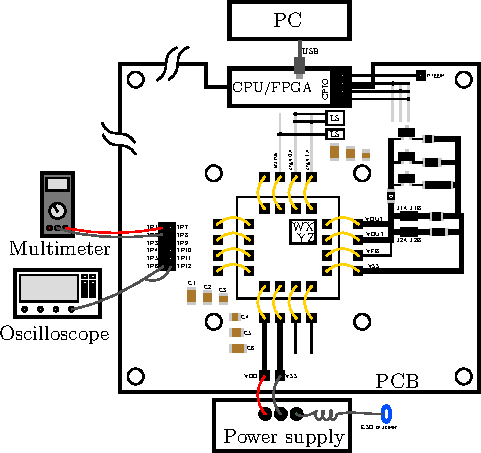
\includegraphics[width=0.55\textwidth]{./figures/big.pdf}
%     \end{figure}
% \end{frame}
% 
% \begin{frame}{Sanity checks: short detection via multimeter}
%     \begin{figure} \centering
%         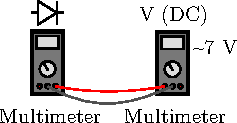
\includegraphics[width=0.55\textwidth]{./figures/multimeter.pdf}
%     \end{figure}
%     This can stress and damage the ASIC pads!
% \end{frame}
% 
% \begin{frame}{Sanity checks: short detection via power supply}
%     \begin{figure} \centering
%         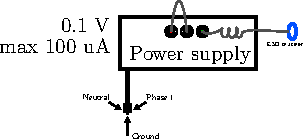
\includegraphics[width=0.55\textwidth]{./figures/power_supply_limit.pdf}
%     \end{figure}
%     To ensure the current protection works, short the supply and monitor the current.
% \end{frame}
% 
% \begin{frame}{Sanity checks: short detection via power supply}
%     \vspace{-0.5cm}
%   \begin{columns}
%       \begin{column}{0.45\textwidth}
%         \begin{itemize}
%             \item Monitor the current on the power supply.
%             \item This also indicates if any VSS is open.
%             \item Connections are actually done to the test points!
%         \end{itemize}
%       \end{column}
%       \begin{column}{0.52\textwidth}
%         \begin{figure} \centering
%             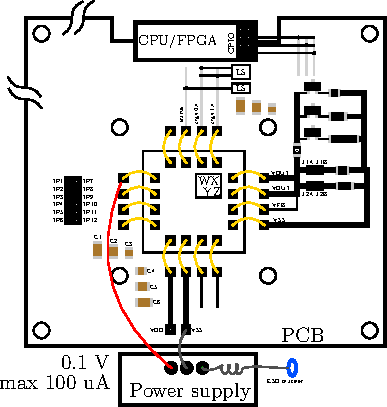
\includegraphics[width=0.9\textwidth]{./figures/short_check1.pdf}
%         \end{figure}
%       \end{column}
%   \end{columns}
% \end{frame}
% 
% \begin{frame}{Sanity checks: short detection via power supply}
%     \vspace{-0.5cm}
%   \begin{columns}
%       \begin{column}{0.45\textwidth}
%         \begin{itemize}
%             \item Monitor the current on the power supply.
%             \item This also indicates if any VSS is open.
%             \item Connections are actually done to the test points!
%             \item Cycle through all the pads.
%         \end{itemize}
%       \end{column}
%       \begin{column}{0.52\textwidth}
%         \begin{figure} \centering
%             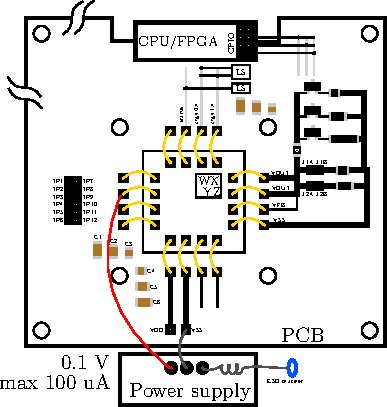
\includegraphics[width=0.9\textwidth]{./figures/short_check2.pdf}
%         \end{figure}
%       \end{column}
%   \end{columns}
% \end{frame}
% 
% 
% 
% %%%%%%%%%%%%%%%%%%%%%%%%%%%%%%%%%%%%%%%%%%%%%%%%%%%%%%%%%%%%%%%%%%%%%%%%%%%%%%%%
% \section{Power-up}
% \begin{frame}[SectionTitlepage]{Power-up}
% \end{frame}
% %%%%%%%%%%%%%%%%%%%%%%%%%%%%%%%%%%%%%%%%%%%%%%%%%%%%%%%%%%%%%%%%%%%%%%%%%%%%%%%%
% 
% \begin{frame}{Power-up I}
%   \vspace{-0.3cm}
%   \begin{columns}
%       \hspace{0.4cm}
%       \begin{column}{0.45\textwidth}
%         \begin{enumerate}
%             \item Connect the power supply with a conservative maximum current and nominal voltage.
%             \item Measure all the test points and internal nets.
%             \item Power your CPU.
%             \item Perform read and write operations to your embedded system.
%         \end{enumerate}
%       \end{column}
%       \begin{column}{0.52\textwidth}
%         \begin{figure} \centering
%             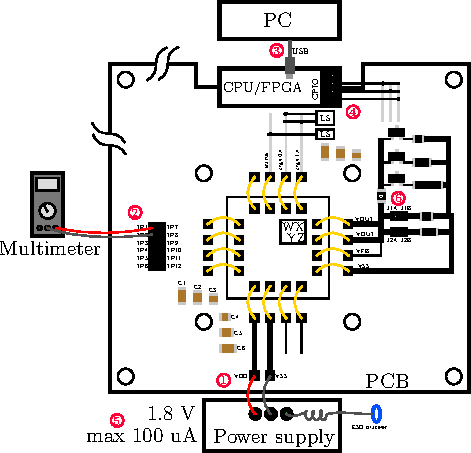
\includegraphics[width=0.9\textwidth]{./figures/big_powerup.pdf}
%         \end{figure}
%       \end{column}
%   \end{columns}
% \end{frame}
% 
% \begin{frame}{Power-up II}
%   \vspace{-0.3cm}
%   \begin{columns}
%       \hspace{0.4cm}
%       \begin{column}{0.45\textwidth}
%         \begin{enumerate}
%             \setcounter{enumi}{4}
%             \item Raise the current limit.
%             \item Exercise different loads and ensure a proper behavior.
%         \end{enumerate}
%       \end{column}
%       \begin{column}{0.52\textwidth}
%         \begin{figure} \centering
%             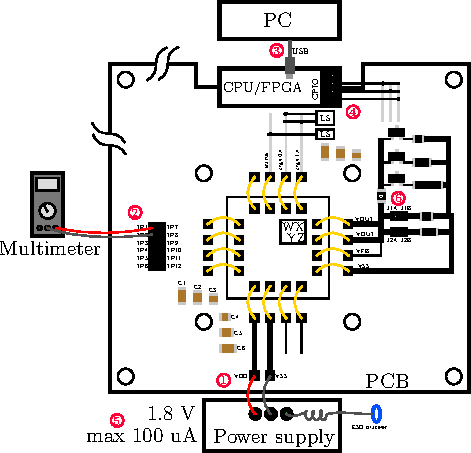
\includegraphics[width=0.9\textwidth]{./figures/big_powerup.pdf}
%         \end{figure}
%       \end{column}
%   \end{columns}
% \end{frame}
% 
% 
% 
% 
% %%%%%%%%%%%%%%%%%%%%%%%%%%%%%%%%%%%%%%%%%%%%%%%%%%%%%%%%%%%%%%%%%%%%%%%%%%%%%%%%
% \section{Characterization}
% \begin{frame}[SectionTitlepage]{Characterization}
% \end{frame}
% %%%%%%%%%%%%%%%%%%%%%%%%%%%%%%%%%%%%%%%%%%%%%%%%%%%%%%%%%%%%%%%%%%%%%%%%%%%%%%%%
% 
% \begin{frame}{Characterization: $I_Q$}
%   \vspace{-0.7cm}
%   \begin{columns}
%       \hspace{0.4cm}
%       \begin{column}{0.4\textwidth}
%         \begin{enumerate}
%             \item Ensure the output is floating (no load).
%             \item Pick a suitable resistor to get a measurable voltage drop, but not too large to power off the LDO.
%         \end{enumerate}
%       \end{column}
%       \begin{column}{0.55\textwidth}
%         \begin{figure} \centering
%             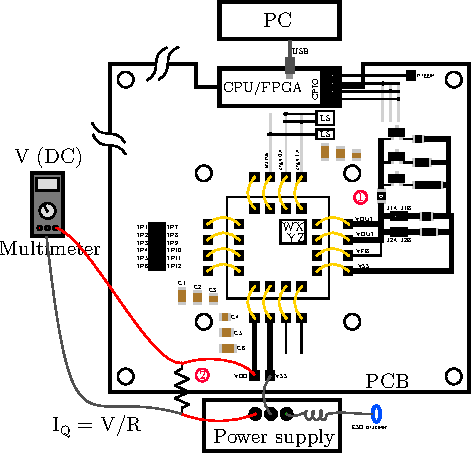
\includegraphics[width=0.95\textwidth]{./figures/meas_iq.pdf}
%         \end{figure}
%       \end{column}
%   \end{columns}
% \end{frame}
% 
% \begin{frame}{Characterization: noise}
%   \vspace{-0.7cm}
%   \begin{columns}
%       \hspace{0.4cm}
%       \begin{column}{0.4\textwidth}
%         \begin{enumerate}
%             \item Perform an FFT on the transient waveform, report the voltage spectral density.
%         \end{enumerate}
%       \end{column}
%       \begin{column}{0.53\textwidth}
%         \begin{figure} \centering
%             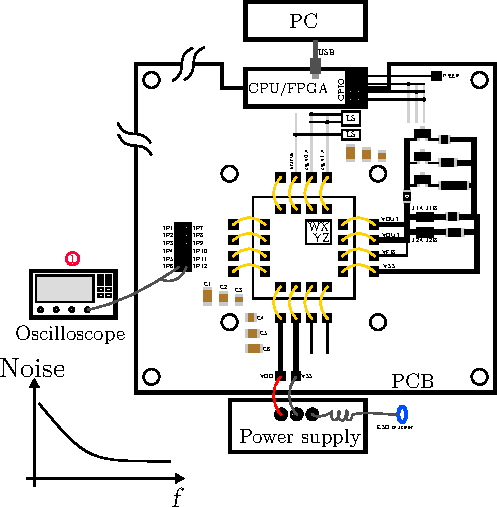
\includegraphics[width=0.95\textwidth]{./figures/meas_noise.pdf}
%         \end{figure}
%       \end{column}
%   \end{columns}
% \end{frame}
% 
% \begin{frame}{Characterization: minimum dropout \cite{Kim_SSCM}}
%   \vspace{-0.7cm}
%   \begin{columns}
%       \hspace{0.4cm}
%       \begin{column}{0.35\textwidth}
%         \begin{enumerate}
%             \item Sweep $V_{in}$
%             \item Sweep $I_\text{load}$.
%             \item Measure $V_{out}$.
%         \end{enumerate}
%       \end{column}
%       \begin{column}{0.6\textwidth}
%         \begin{figure} \centering
%             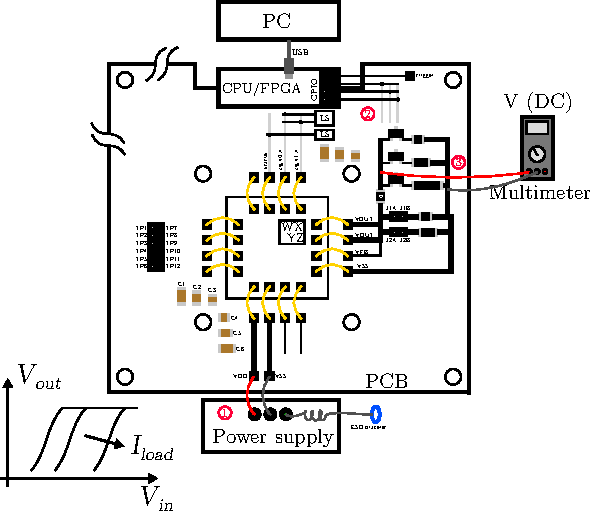
\includegraphics[width=0.95\textwidth]{./figures/meas_loadVout.pdf}
%         \end{figure}
%       \end{column}
%   \end{columns}
% \end{frame}
% 
% \begin{frame}{Characterization: load regulation}
%   \vspace{-0.7cm}
%   \begin{columns}
%       \hspace{0.4cm}
%       \begin{column}{0.35\textwidth}
%         \begin{enumerate}
%             \item Measure in advance the loads precisely.
%             \item Toggle the load.
%             \item Capture the transient response. Can use the trigger signal.
%         \end{enumerate}
%       \end{column}
%       \begin{column}{0.6\textwidth}
%         \begin{figure} \centering
%             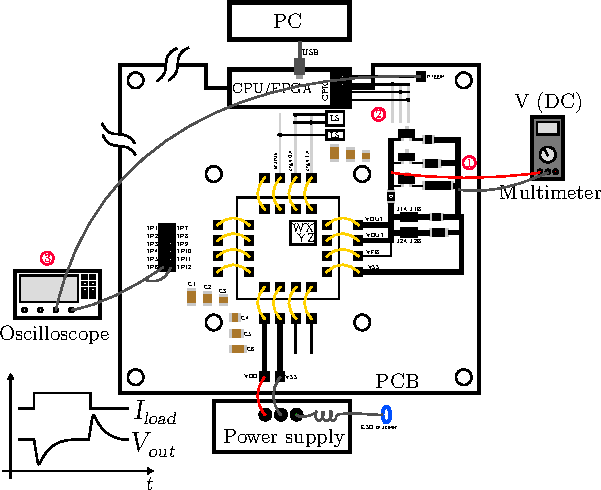
\includegraphics[width=0.95\textwidth]{./figures/meas_transient.pdf}
%         \end{figure}
%       \end{column}
%   \end{columns}
% \end{frame}
% 
% \begin{frame}{Characterization: line regulation (PSRR)}
%   \vspace{-0.7cm}
%   \begin{columns}
%       \hspace{0.4cm}
%       \begin{column}{0.4\textwidth}
%         \begin{enumerate}
%             \item Add an AC component on $V_{in}$
%             \item Measure the spectrum on $V_{out}$.
%         \end{enumerate}
%       \end{column}
%       \begin{column}{0.55\textwidth}
%         \begin{figure} \centering
%             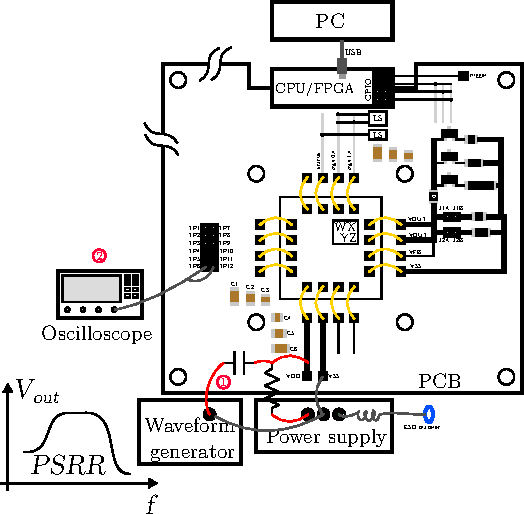
\includegraphics[width=0.95\textwidth]{./figures/meas_PSRR.pdf}
%         \end{figure}
%       \end{column}
%   \end{columns}
% \end{frame}
% 
% 



%%%%%%%%%%%%%%%%%%%%%%%%%%%%%%%%%%%%%%%%%%%%%%%%%%%%%%%%%%%%%%%%%%%%%%%
%%%%%%%%%%%%%%%%%%%%%%%%%%%%%%%%%%%%%%%%%%%%%%%%%%%%%%%%%%%%%%%%%%%%%%%
%%%%%%%%%%%%%%%%%%%%%%%%%%%%%%%%%%%%%%%%%%%%%%%%%%%%%%%%%%%%%%%%%%%%%%%


\begin{frame}[allowframebreaks]{References}
    \printbibliography
\end{frame}


\end{document}
